\chapter{运行时可定制调度的沙箱机制实现}\label{chap:control_zone}

为解决单一调度机制与多样混部场景的问题,本章设计实现了Contorl Zone,一种面向混部场景的调度动态可定制沙箱。Control Zone基于KVM虚拟机实现,允许用户基于Control Tower任务调度框架定制调度策略容器与混部应用共同部署,一方面,针对不同混部场景,允许用户自由地选择合适的调度策略容器,另一方面,允许用户根据混部应用的变化,在运行时对调度策略容器进行动态修改,而在不同的Control Zone之间,允许用户借助丰富的资源隔离手段,来定制对混部应用的资源保护。

\section{Control Zone设计}

% 概述 -> 设计思路

% 介绍 Control Zone 的概念
% - 面对什么场景
% - 存在哪些问题
%   - 复杂的硬件环境
%   - 复杂的软件环境
% - 针对每个问题的解决方式
% - 设计目标

在航空领域,Control Zone指受控空域的一部分,通常在机场的周围,保护进出机场的的空中交通,而在Control Zone之中,由Control Tower进行客机起降的调度。本文借用Control Zone概念设计沙箱系统,在外层提供足够强的隔离性,而在内层则提供运行时可定制的任务调度框架Control Tower,Control Zone包含如下特性:

\begin{itemize}
    \item \textbf{轻量级虚拟机}:Control Zone使用虚拟机来提供更强的隔离性,而轻量化体现在两方面,一方面采用轻量化的Hypervisor,提供更快的虚拟机启动速度与内存占用, 另一方使用最小化Guest内核及精简根文件系统,提供快速的系统引导与基本的系统功能。
    \item \textbf{容器化的任务}:Control Zone包含一个最小化的容器环境与容器运行时,支持大量容器化应用的运行,同时享容器镜像与目录文件能够在不同的Control Zone之间共享,支持跨Control Zone的任务协作。
    \item \textbf{可动态定制的调度器}:Control Zone支持Control Tower调度框架,运行以容器方式打包的调度策略。Control Zone提供了基础的调度策略容器,同时,调度策略容器与任务容器的管理方式相同,同样支持运行时的修改与切换。
    \item \textbf{可观测性基础设施}:沙箱系统包含了一个围绕虚拟机的可观测性系统,能够从Host、Hypervisor、App三个层次以虚拟机为粒度采集丰富的指标,并提供实时监测与离线分析功能来全面地分析虚拟机及其中任务的性能。
\end{itemize}

\begin{figure}[!htbp]
    \centering
    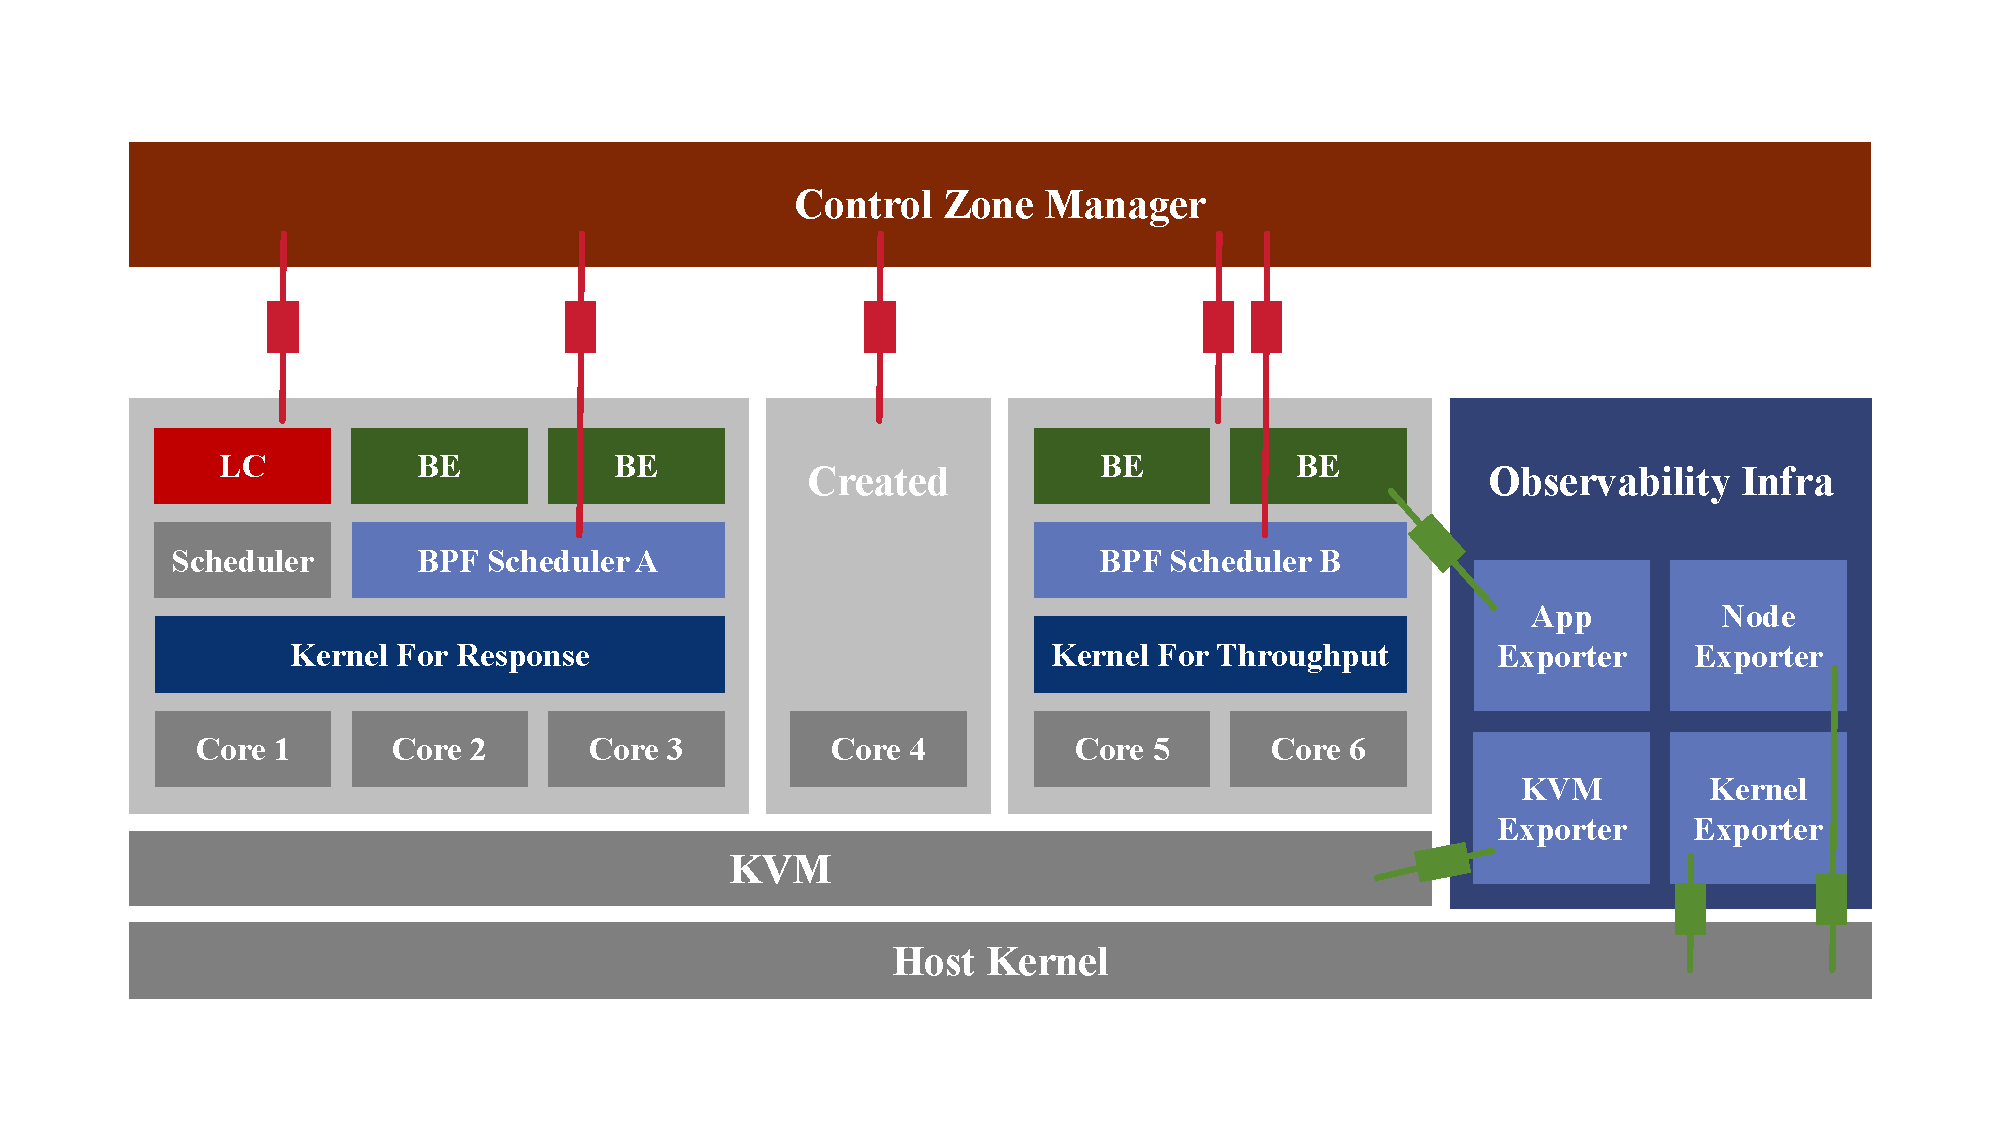
\includegraphics[width=1.0\textwidth]{controlzone_arch}
    \bicaption{\quad Control Zone基本架构}{\quad Control Zone Architectural}
    \label{fig:controlzone_arch}
\end{figure}
 
Control Zone整体架构如图~\ref{fig:controlzone_arch}所示,其中,管理器负责进行Control Zone的管理,提供隔离环境的定制能力,并可以根据混部任务的属性动态地对BPF Scheduler进行修改,可观测性基础设置则能够与各层次的系统组件交互,以采集全面的虚拟机指标信息。

对于混部场景下的硬件特性差异的挑战,一方面,Control Zone能够利用虚拟化提供的抽象层屏蔽底层硬件的差异,另一方面,Control Zone可以根据配置的硬件特性选择合适的Control Tower任务调度策略,并能够在硬件特性变化时切换另一个合适的任务调度策略,过程中不需要中断虚拟机的执行。

对于混部场景下软件需求差异的挑战,首先,针对高优先级任务的特性,可以选择匹配的内核来满足任务在响应度或吞吐量上的需求。其次,针对差异的混部场景,则能够选择场景定制的任务调度策略来处理QoS保障问题,同时,考虑混部应用的负载的动态特性,一方面可以通过eBPF监测应用的负载,另一方面可以在不同的阶段切换不同的任务调度策略来实现灵活的QoS保障策略。

\section{Control Zone实现}

\subsection{Control Zone组成}

% 优化图例
% 使用中文名称,体现功能
% Control Zone组成,阐述各个组成部分所做的功能,希望实现的目标
% - czctrl: Control Zone管理
% - czdaemon: 容器管理
%   - chsd: 调度策略管理
% - observity: 可观测性

运行时可定制调度的沙箱包括Control Zone管理、应用管理及可观测性三个主要部分。如图~\ref{fig:cz_components}所示,用户通过czyaml配置文件来定义一个Control Zone,而Control Zone的管理主要czctrl、czmanager及虚拟化运行时三个组件协作完成。每个Control Zone都运行有一个czdaemon,并与czctrl、czmanager协作实现应用管理。可观测性沿用了第三章中设计的在线指标监测系统,通过与czmanager的协作完成对于虚拟机的监控。镜像存储服务负责管理OCI镜像,并在Control Zone管理的各个阶段提供镜像存储服务。

\begin{figure}[!htbp]
    \centering
    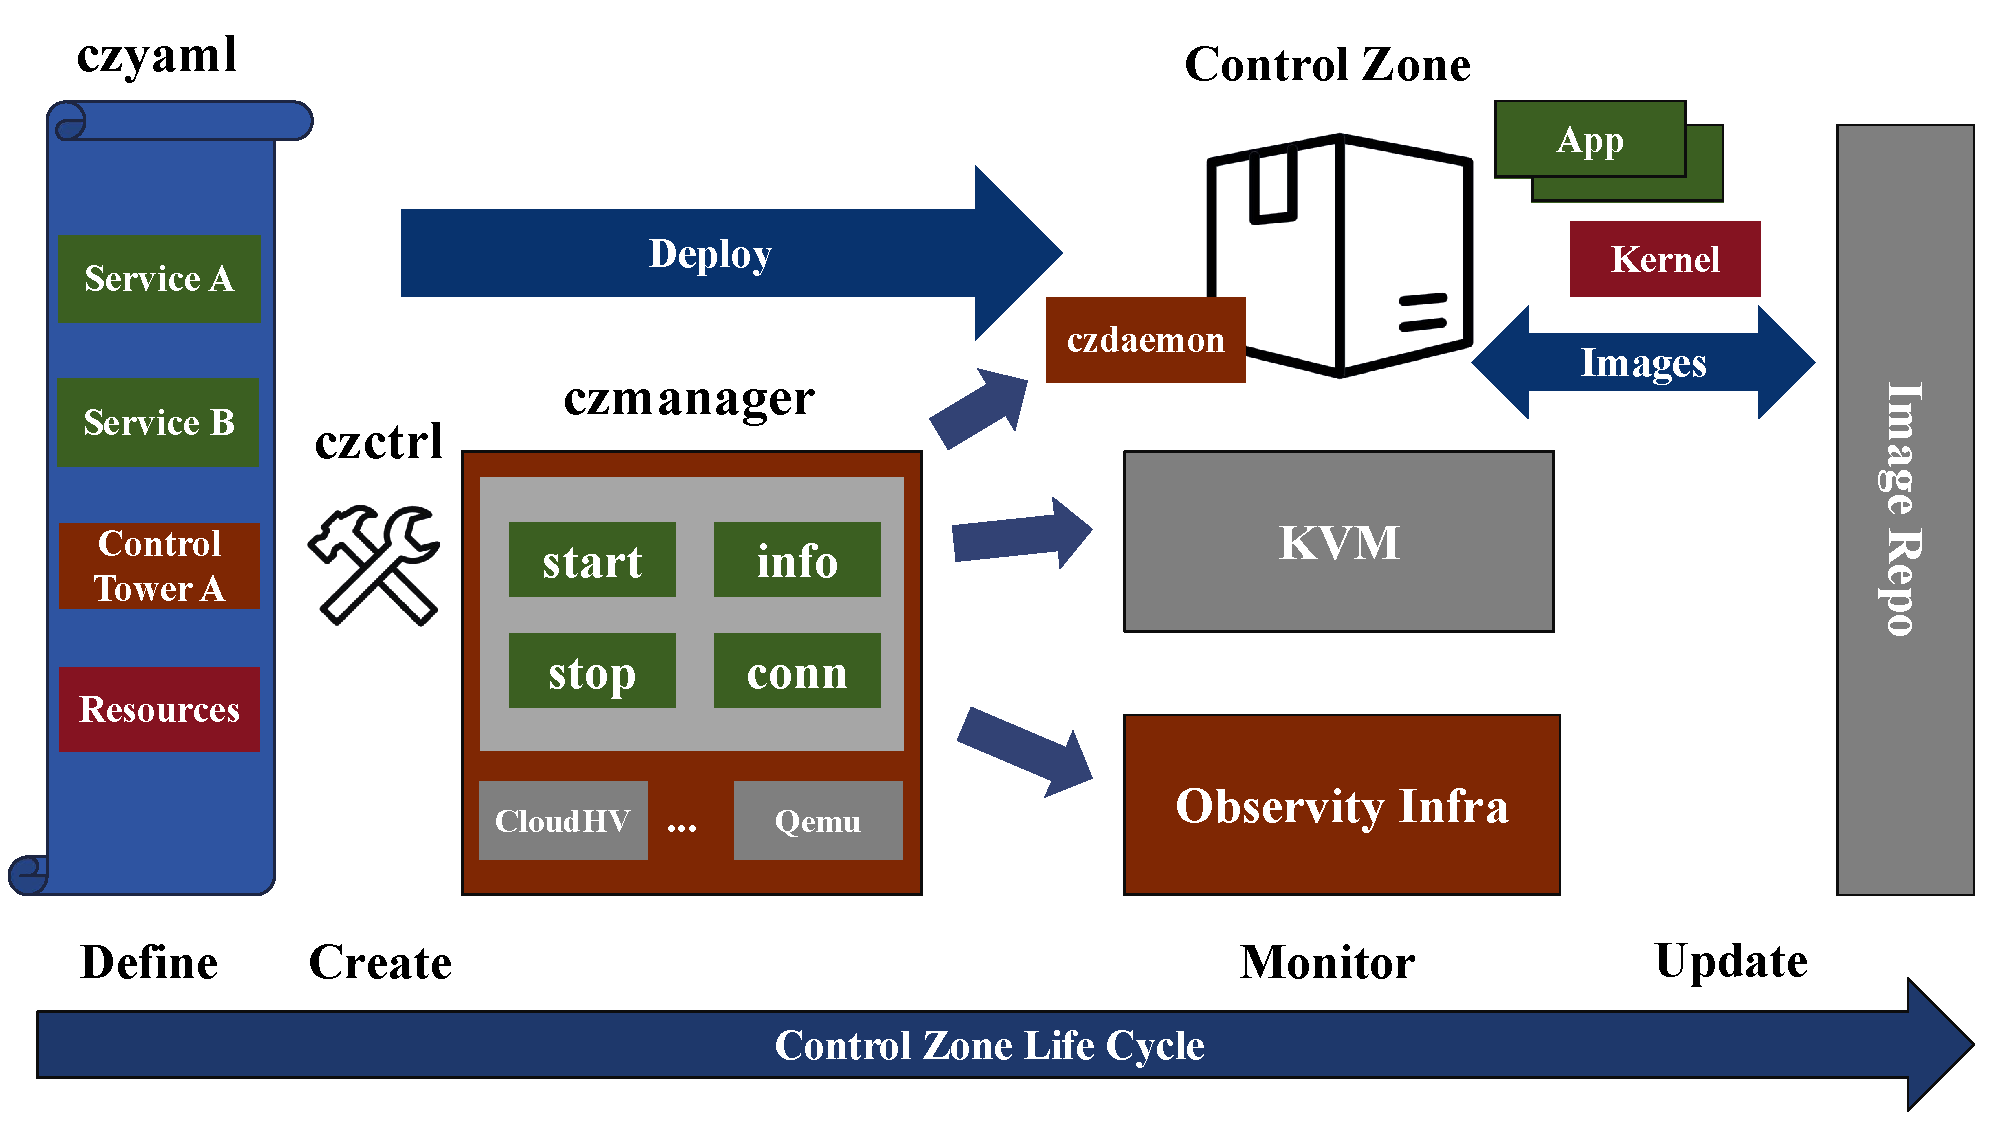
\includegraphics[width=0.9\textwidth]{cz_components}
    \bicaption{\quad Control Zone组件结构}{\quad Components of Control Zone}
    \label{fig:cz_components}
\end{figure}

\begin{itemize}
    \item \textbf{czyaml}:Control Zone定义。czyaml包含Meta、Guest、Resource三部分,其中Meta包含一些元数据,用以区分不同的Control Zone。Guest部分则用于声明运行环境,包括使用的系统、调度器及根文件系统。Resource部分用于声明隔离的资源,包括常见的CPU、Memory以及Intel RDT子系统中的LLC和内存带宽。
    \item \textbf{czmanager}:Control Zone管理。czmanager负责Control Zone的实际管理, 包括创建、查看、启动、暂停、更新以及清除等完善的生命周期管理。过程中czmanager主要负责维护Control Zone的状态,并协同底层虚拟化运行时实现最终的虚拟机管理。而在可观测性上,czmanager利用了虚拟机各层次的信息生成监控配置,并与可观测性基础设施协作以实现Control Zone的持续监控。资源管理上,czmanager主要与虚拟化运行时、Linux Resctrl及Cgroup子系统交互,根据czyaml中的定义实现Control Zone的资源隔离。
    \item \textbf{czdaemon}:Control Zone守护程序。czdaemon运行在每个Control Zone之中,在启动阶段主要用来信息获取与状态探测。而在启动完成之后,作为Control Zone内外沟通的桥梁,对外与czmanager交互,以接收命令,对内则直接与容器运行时交互,实现镜像及容器的管理。
    \item \textbf{czctrl}:用户命令行工具。czctrl是所有请求的入口,能够解析用户输入的命令并验证czyaml配置,随后再与czmanager交互以达成用户管理Control Zone和任务的目的。
    \item \textbf{镜像存储服务}:容器及其他静态资源管理。应用与Control Tower任务调度策略都以OCI容器镜像的形式保存在镜像存储服务中,并通过容器的形式运行,同时为方便其他静态资源的管理,预编译内核及根文件系统也保存在精简容器镜像的中交给镜像存储服务管理。
\end{itemize}

\subsection{Control Zone流程}

% 要解决的问题,以及解决的问题的思路

% Control Zone Yaml
% Control Zone关键流程的执行过程
% - start
% - stop 
% - update
% - remove
% Control Zone容器的管理流程
% - add
% - delete
% Control Zone调度的流程
% - czctrl的资源限制
% - chsd的策略控制
% - sched ext的策略控制

Control Zone Yaml提供了丰富的配置选项,允许用户自定义沙箱的基本配置,并提供丰富的资源隔离声明。

\begin{itemize}
    \item \textbf{基础配置}:Control Zone基础配置如表~\ref{tab:cz_meta_config}所示,首先,在Guest环境上,Control Zone提供了Response、Throughput两种基本内核,用户可根据需要进行选择。为加快启动速度,Control Zone默认不使用initramfs,同时提供了基于Alpine的轻量化rootfs,其中包含基础的软件运行环境,用户也可以根据需要进行修改。其次,在应用管理上,Control Zone使用Pod Yaml来描述混部任务的部署需求,其中Control Tower调度器与常规应用一样基于容器部署,并包含在Pod Yaml中。

\begin{table}[H]
    \bicaption{\quad Control Zone Meta 配置}{\quad Control Zone Meta Config}% caption
    \label{tab:cz_meta_config}
    \footnotesize% fontsize
    \setlength{\tabcolsep}{4pt}% column separation
    \renewcommand{\arraystretch}{1.25}% row space 
    \centering
    \begin{tabular}{lc}
        \hline
        %\multicolumn{num_of_cols_to_merge}{alignment}{contents} \\
        %\cline{i-j}% partial hline from column i to column j
        配置 & 说明\\
        \hline
        name & Control Zone名称 \\
        workdir & Control Zone工作目录,存放日志及其他配置 \\
        share\_folder(可选) & 额外共享给Control Zone的目录 \\
        label & 标签,数个key-value对 \\
        vrun & 虚拟机运行时,可选CloudHypervisor、Qemu或Libvirtd \\
        initramfs(可选) & 初始化内存文件系统,默认情况下不使用 \\
        rootfs(可选) & Control Zone使用的根文件系统,从镜像存储拉取\\
        kcmdline(可选) & 内核的运行命令 \\
        pods(可选) & Pod 配置 \\
        \hline
    \end{tabular}
\end{table}

    \item \textbf{资源配置}:KVM虚拟机是一种特殊的进程,Control Zone在创建虚拟机的过程中,会为vCPU及emulator线程创建Cgroup与Resctrl Monitor Group来方便进行资源管理,具体的资源配置选项如表~\ref{tab:cz_cgroup_config}所示。首先,基于Cgroup,用户可以配置vCPU在pCPU上的资源使用,围绕CPU亲和性与CPU时间片使用展开。其次,通过Resctrl子系统,也可以为整个虚拟机线程组配置LLC掩码,以进行Cache资源的隔离。

\begin{table}[H]
    \bicaption{\quad Control Zone Resource 配置}{\quad Control Zone Resource Config}% caption
    \label{tab:cz_cgroup_config}
    \footnotesize% fontsize
    \setlength{\tabcolsep}{30pt}% column separation
    \renewcommand{\arraystretch}{1.25}% row space 
    \centering
    \begin{tabular}{lc}
        \hline
        %\multicolumn{num_of_cols_to_merge}{alignment}{contents} \\
        %\cline{i-j}% partial hline from column i to column j
        配置 & 说明\\
        \hline
        cpu.max & 最大CPU使用限制 \\
        cpu.max.burst & 最大突发CPU使用限制 \\
        cpuset.cpus & CPU亲和性 \\
        cpuset.mems & 内存节点亲和性 \\
        llc mask& 可用LLC掩码 \\
        \hline
    \end{tabular}
\end{table}

    \item \textbf{Hypervisor配置}:虚拟机硬件通常由Hypervisor模拟,其中如virtio设备等在模拟设备后端驱动上提供了丰富的配置选项。通过Hypervisor提供的调控接口,可以进一步在设备上进行资源隔离的配置,具体配置如表~\ref{tab:cz_hv_config}所示。首先,对于CPU,可以配置提供给虚拟机使用的CPU feature。而对于virtio网络设备和块设备,则可以在收发速度上进行限制。

\begin{table}[H]
    \bicaption{\quad Control Zone Hypervisor 配置}{\quad Control Zone Hypervisor Config}% caption
    \label{tab:cz_hv_config}
    \footnotesize% fontsize
    \setlength{\tabcolsep}{30pt}% column separation
    \renewcommand{\arraystretch}{1.25}% row space 
    \centering
    \begin{tabular}{lc}
        \hline
        %\multicolumn{num_of_cols_to_merge}{alignment}{contents} \\
        %\cline{i-j}% partial hline from column i to column j
        配置 & 说明\\
        \hline
        cpu features& vCPU可用的特性\\
        bw\_size & 设备带宽大小(byte/s)\\
        bw\_one\_time\_burst & 设备突发带宽大小(byte/s)\\
        bw\_refill\_time & 设备带宽恢复时间(ms)\\
        ops\_size & 设备操作速度(op/s)\\
        ops\_one\_time\_burst & 设备突发操作速度(op/s)\\
        ops\_refill\_time & 设备操作速度恢复时间(ms)\\
        \hline
    \end{tabular}
\end{table}

\end{itemize}


运行时可定制调度的沙箱提供了create、start、stop、remove、update四种操作来管理Control Zone的生命周期,在不同操作下Control Zone的状态变化如图~\ref{fig:cz_state}所示,其中 sync 过程由czdaemon完成,而对于不能直接达到的状态,czmanager会试图进行多次状态切花以达到目标状态,而对于不可达的状态,czmanager将会提示操作非法。update操作对于状态的影响取决于所更新的参数,如对内核的修改将要求Control Zone进行重新启动。

\begin{figure}[!htbp]
    \centering
    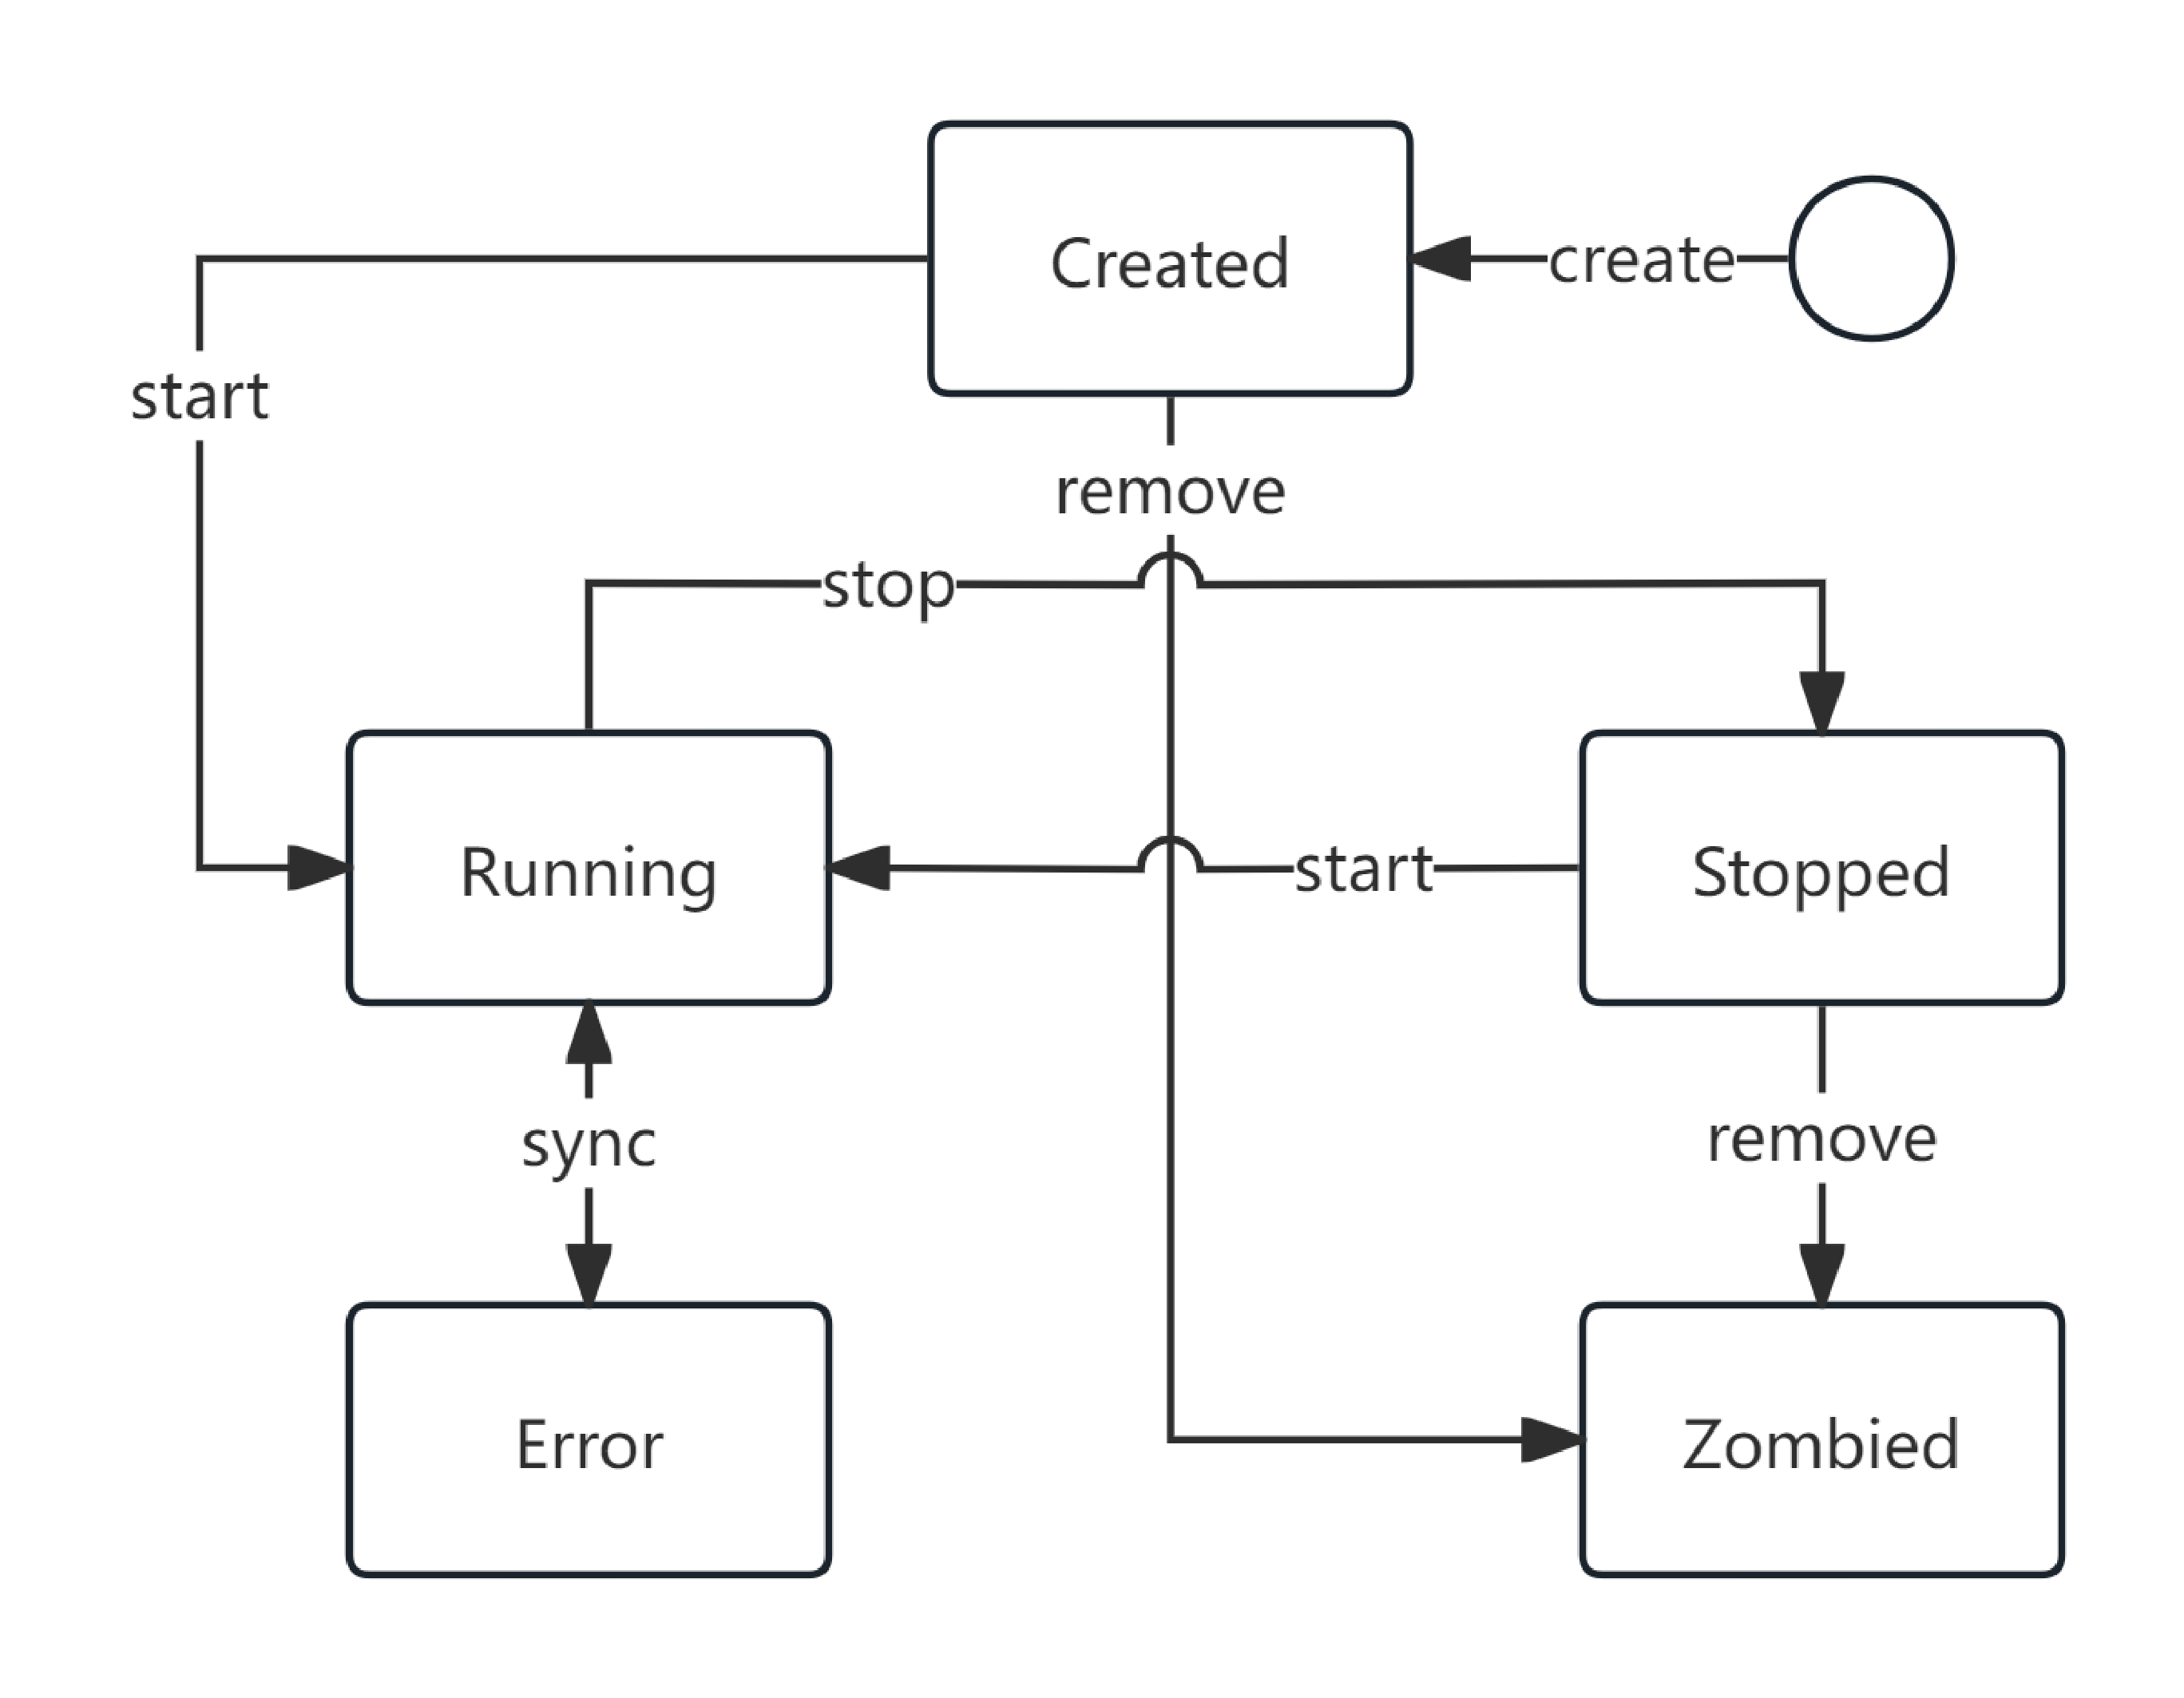
\includegraphics[width=0.6\textwidth]{cz_state}
    \bicaption{\quad Control Zone状态迁移}{\quad State of Control Zone}
    \label{fig:cz_state}
\end{figure}

Control Zone的创建流程如图~\ref{fig:cz_create}所示,过程中首先进行配置的合法性监测,创建过程中的检测主要判断资源是否重复分配,如对于cpuset,czmanager会检查全局的cpu mask来判断cpuset的设置是否合法。随后进行工作目录的创建,用来单独保存每个Control Zone的关键数据,如根文件系统等。创建过程仅为虚拟机的启动做好准备,而并不会启动虚拟机,相当于为虚拟机的启动预留了空间。

\begin{figure}[H]
    \centering
    \begin{subfigure}[b]{0.43\textwidth}
        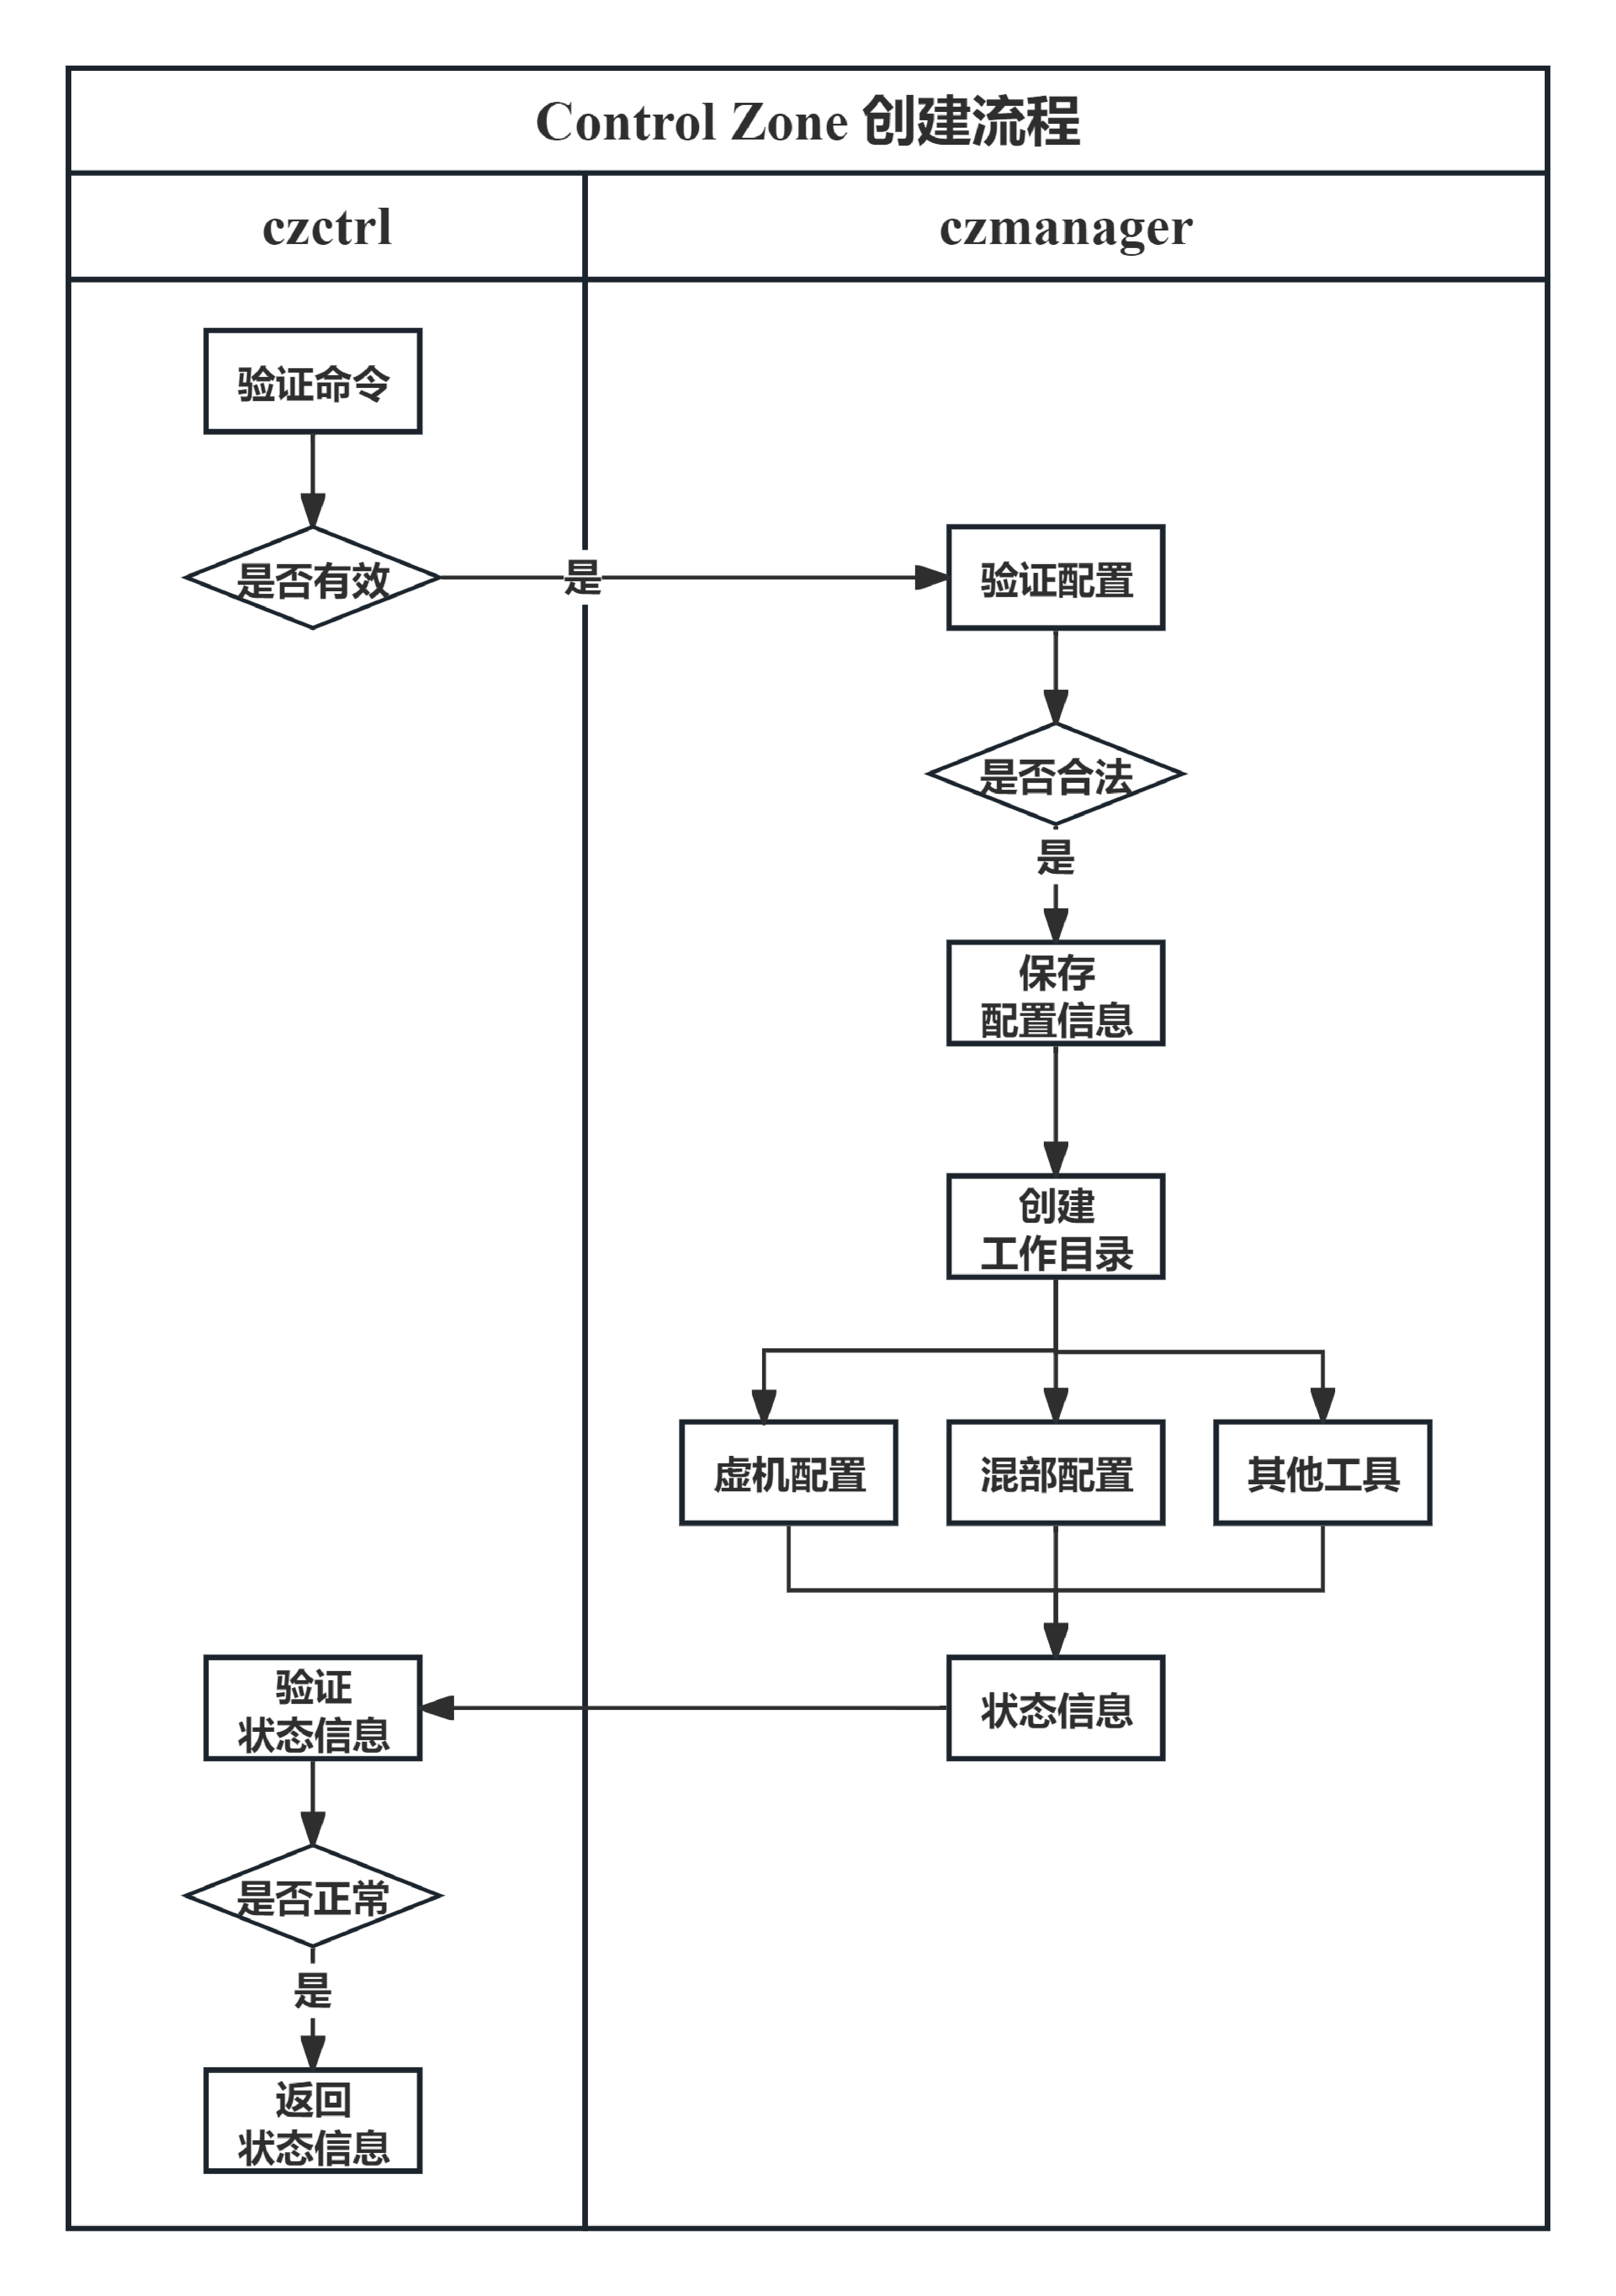
\includegraphics[width=\textwidth]{cz_create}
        \caption{\quad Control Zone创建流程}
        \label{fig:cz_create}
    \end{subfigure}
    \begin{subfigure}[b]{0.56\textwidth}
        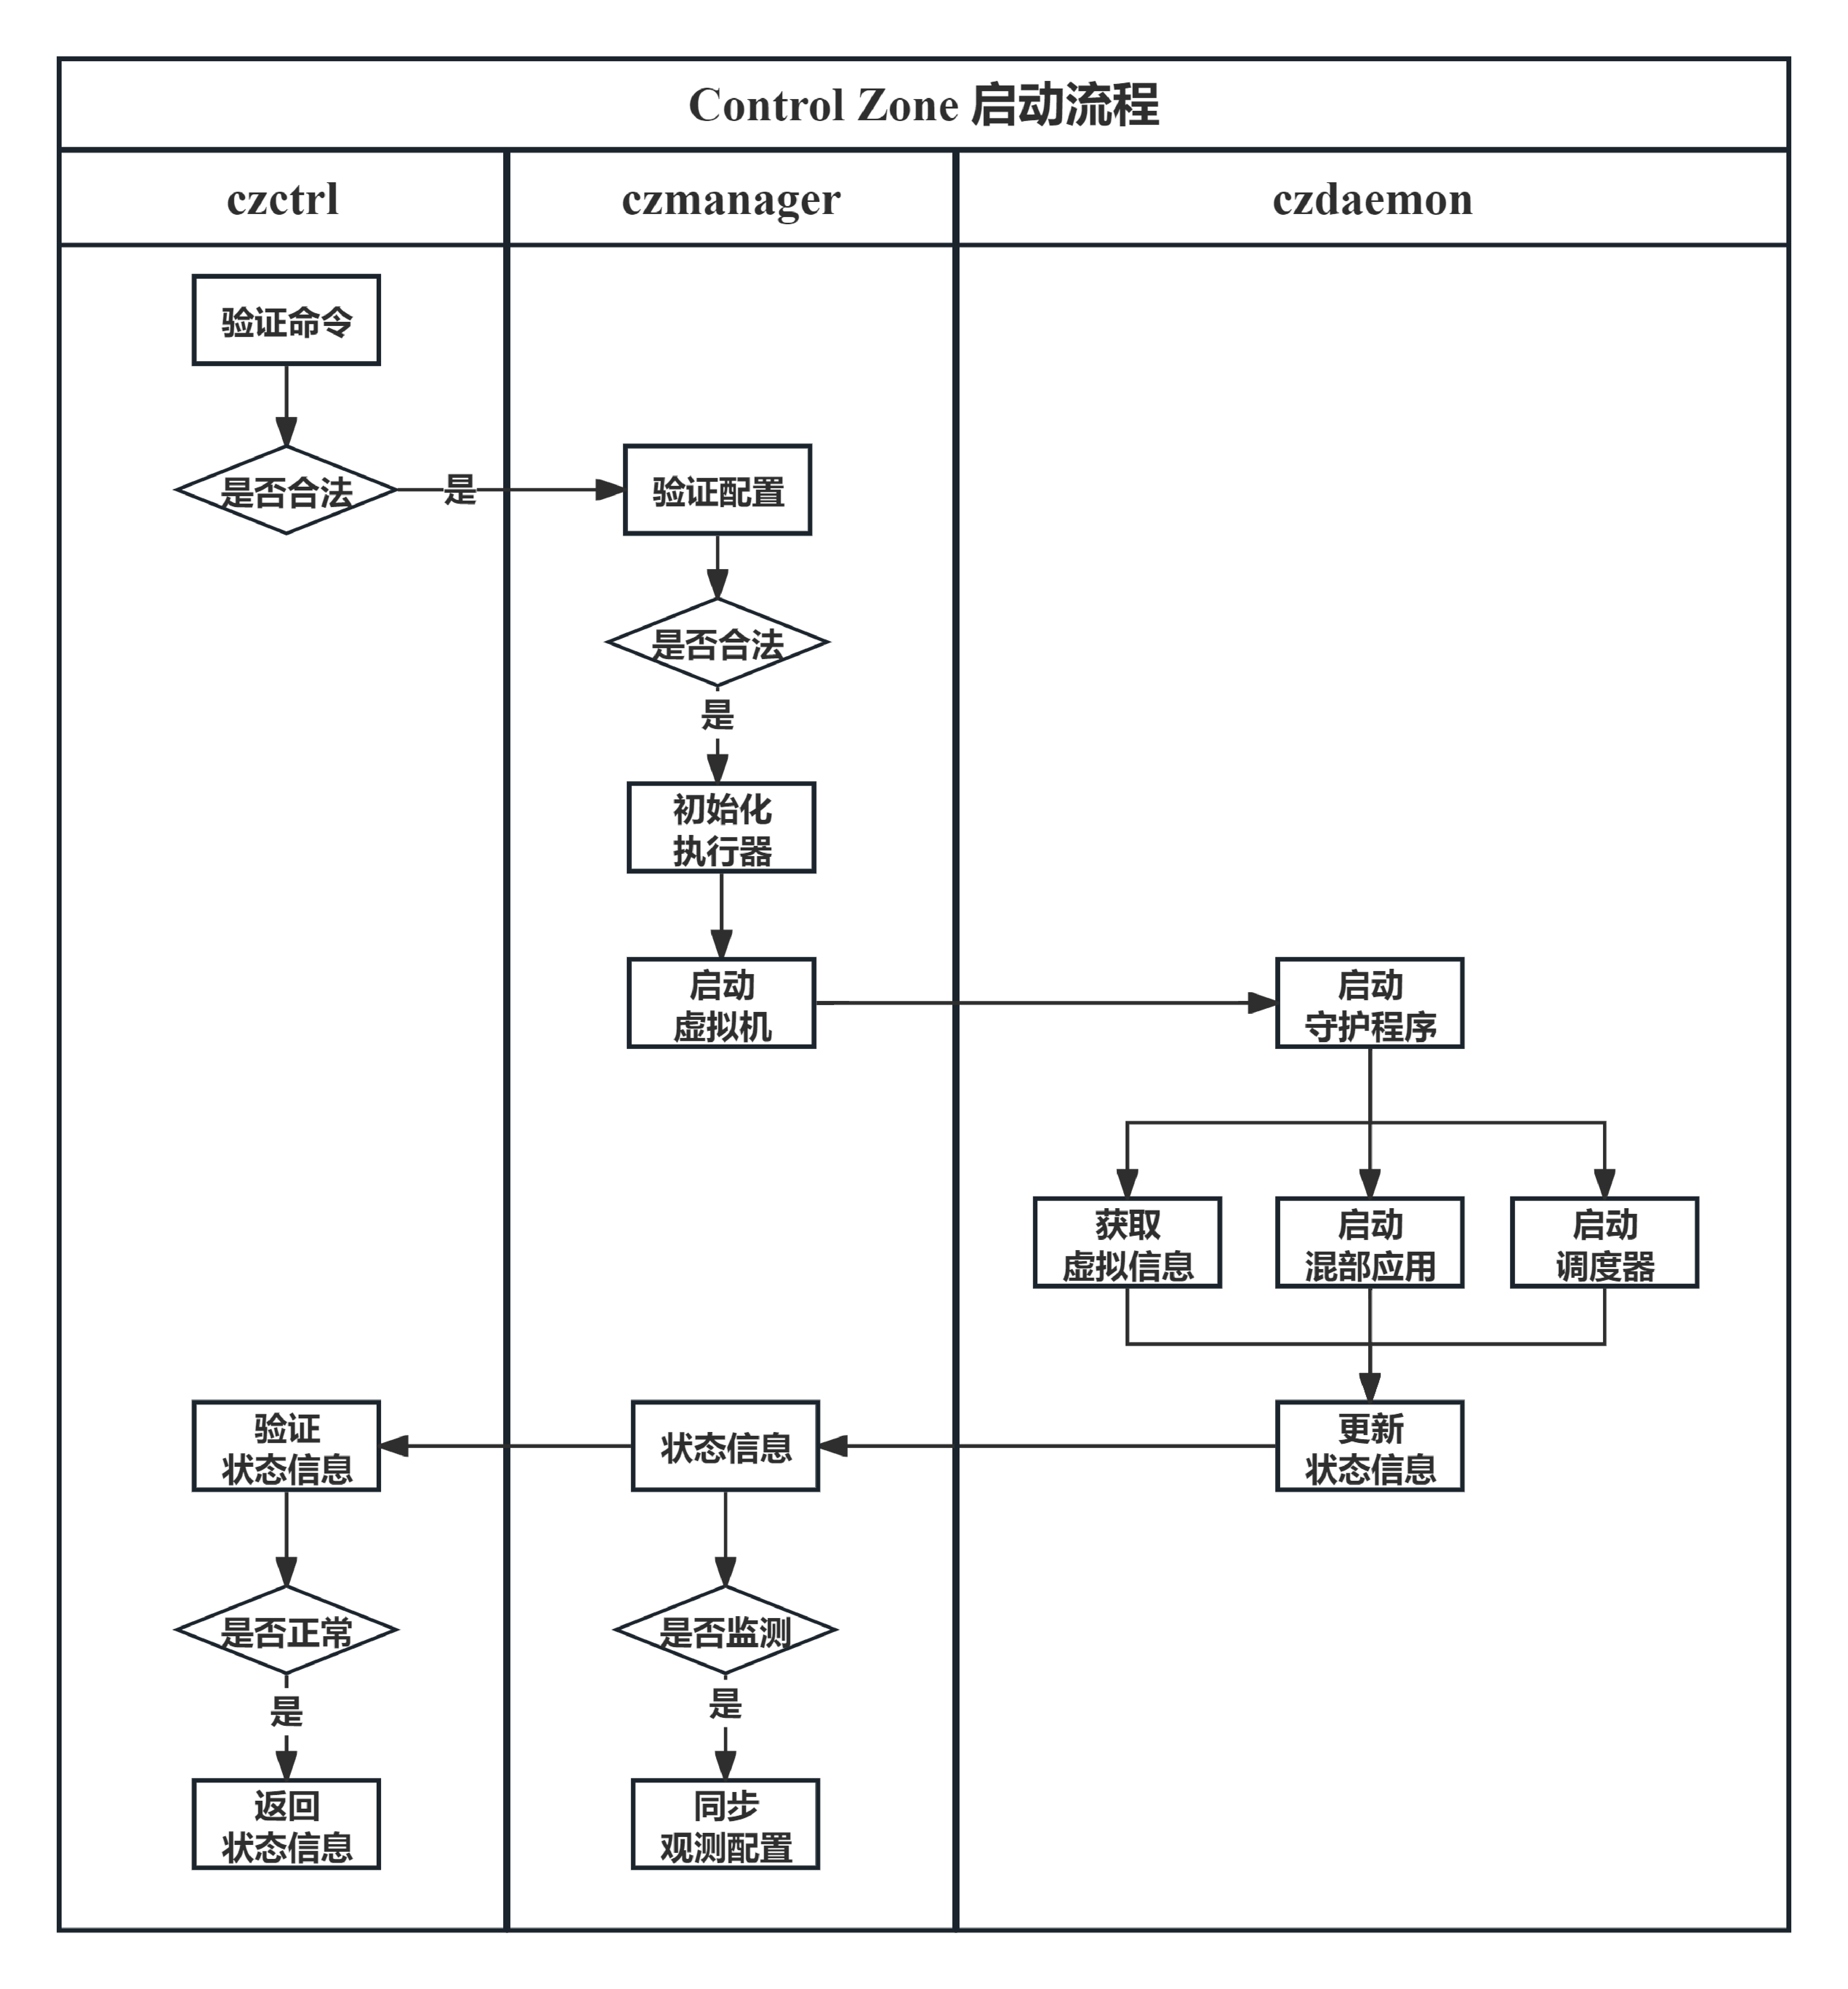
\includegraphics[width=\linewidth]{cz_start}
        \caption{\quad Control Zone启动流程}
        \label{fig:cz_start}
    \end{subfigure}
\bicaption{\quad Control Zone创建与启动流程}{\quad Control Zone creation and startup process}
\label{fig:cz_create_start}
\end{figure}

Control Zone的启动流程如图~\ref{fig:cz_start}所示,过程中首先进行配置的合法性监测,如判断状态迁移是否合法、验证资源是否重复分配,对于一个已经创建的Control Zone,其预留的资源并不是严格进行保护的,因此在启动时其资源可能已经被占用,此时需要涉及重新更新Control Zone的资源配置。而在一切准备就绪以后,czmanager会按照配置要求,调用目标虚拟化运行时来启动虚拟机,而在虚拟机启动完毕之后,czdaemon会检测是否有已经提交的任务,并依次在后台进行执行,随后通知czmanager虚拟机状态的变化,czmanager在收到信号之后,Control Zone的启动过程就完成,而随后czmanager会根据配置来选择为Control Zone同步观测配置。

Control Zone的停止过程如图~\ref{fig:cz_stop}所示,考虑停止之后存在重新启动的可能,因此沙箱采用了较为保守的关闭策略。关闭过程中需要czmanager与czdaemon协同合作,在验证配置之后,czmanager首先会通知czdaemon进行关闭处理,而czdaemon在接收到关闭信号之后,会对当前系统的状态进行保存,如必要的信息、混部应用状态等,再将托管的任务关闭,随后再通知czmanager, 直到此时czmanager才会真正地调用执行器来关闭虚拟机,并在必要时通知可观测性基础设置停止监测。Control Zone停止之后仍然会保有相关的资源记录,便于后续重新启动。

\begin{figure}[H]
    \centering
    \begin{subfigure}[b]{0.46\textwidth}
        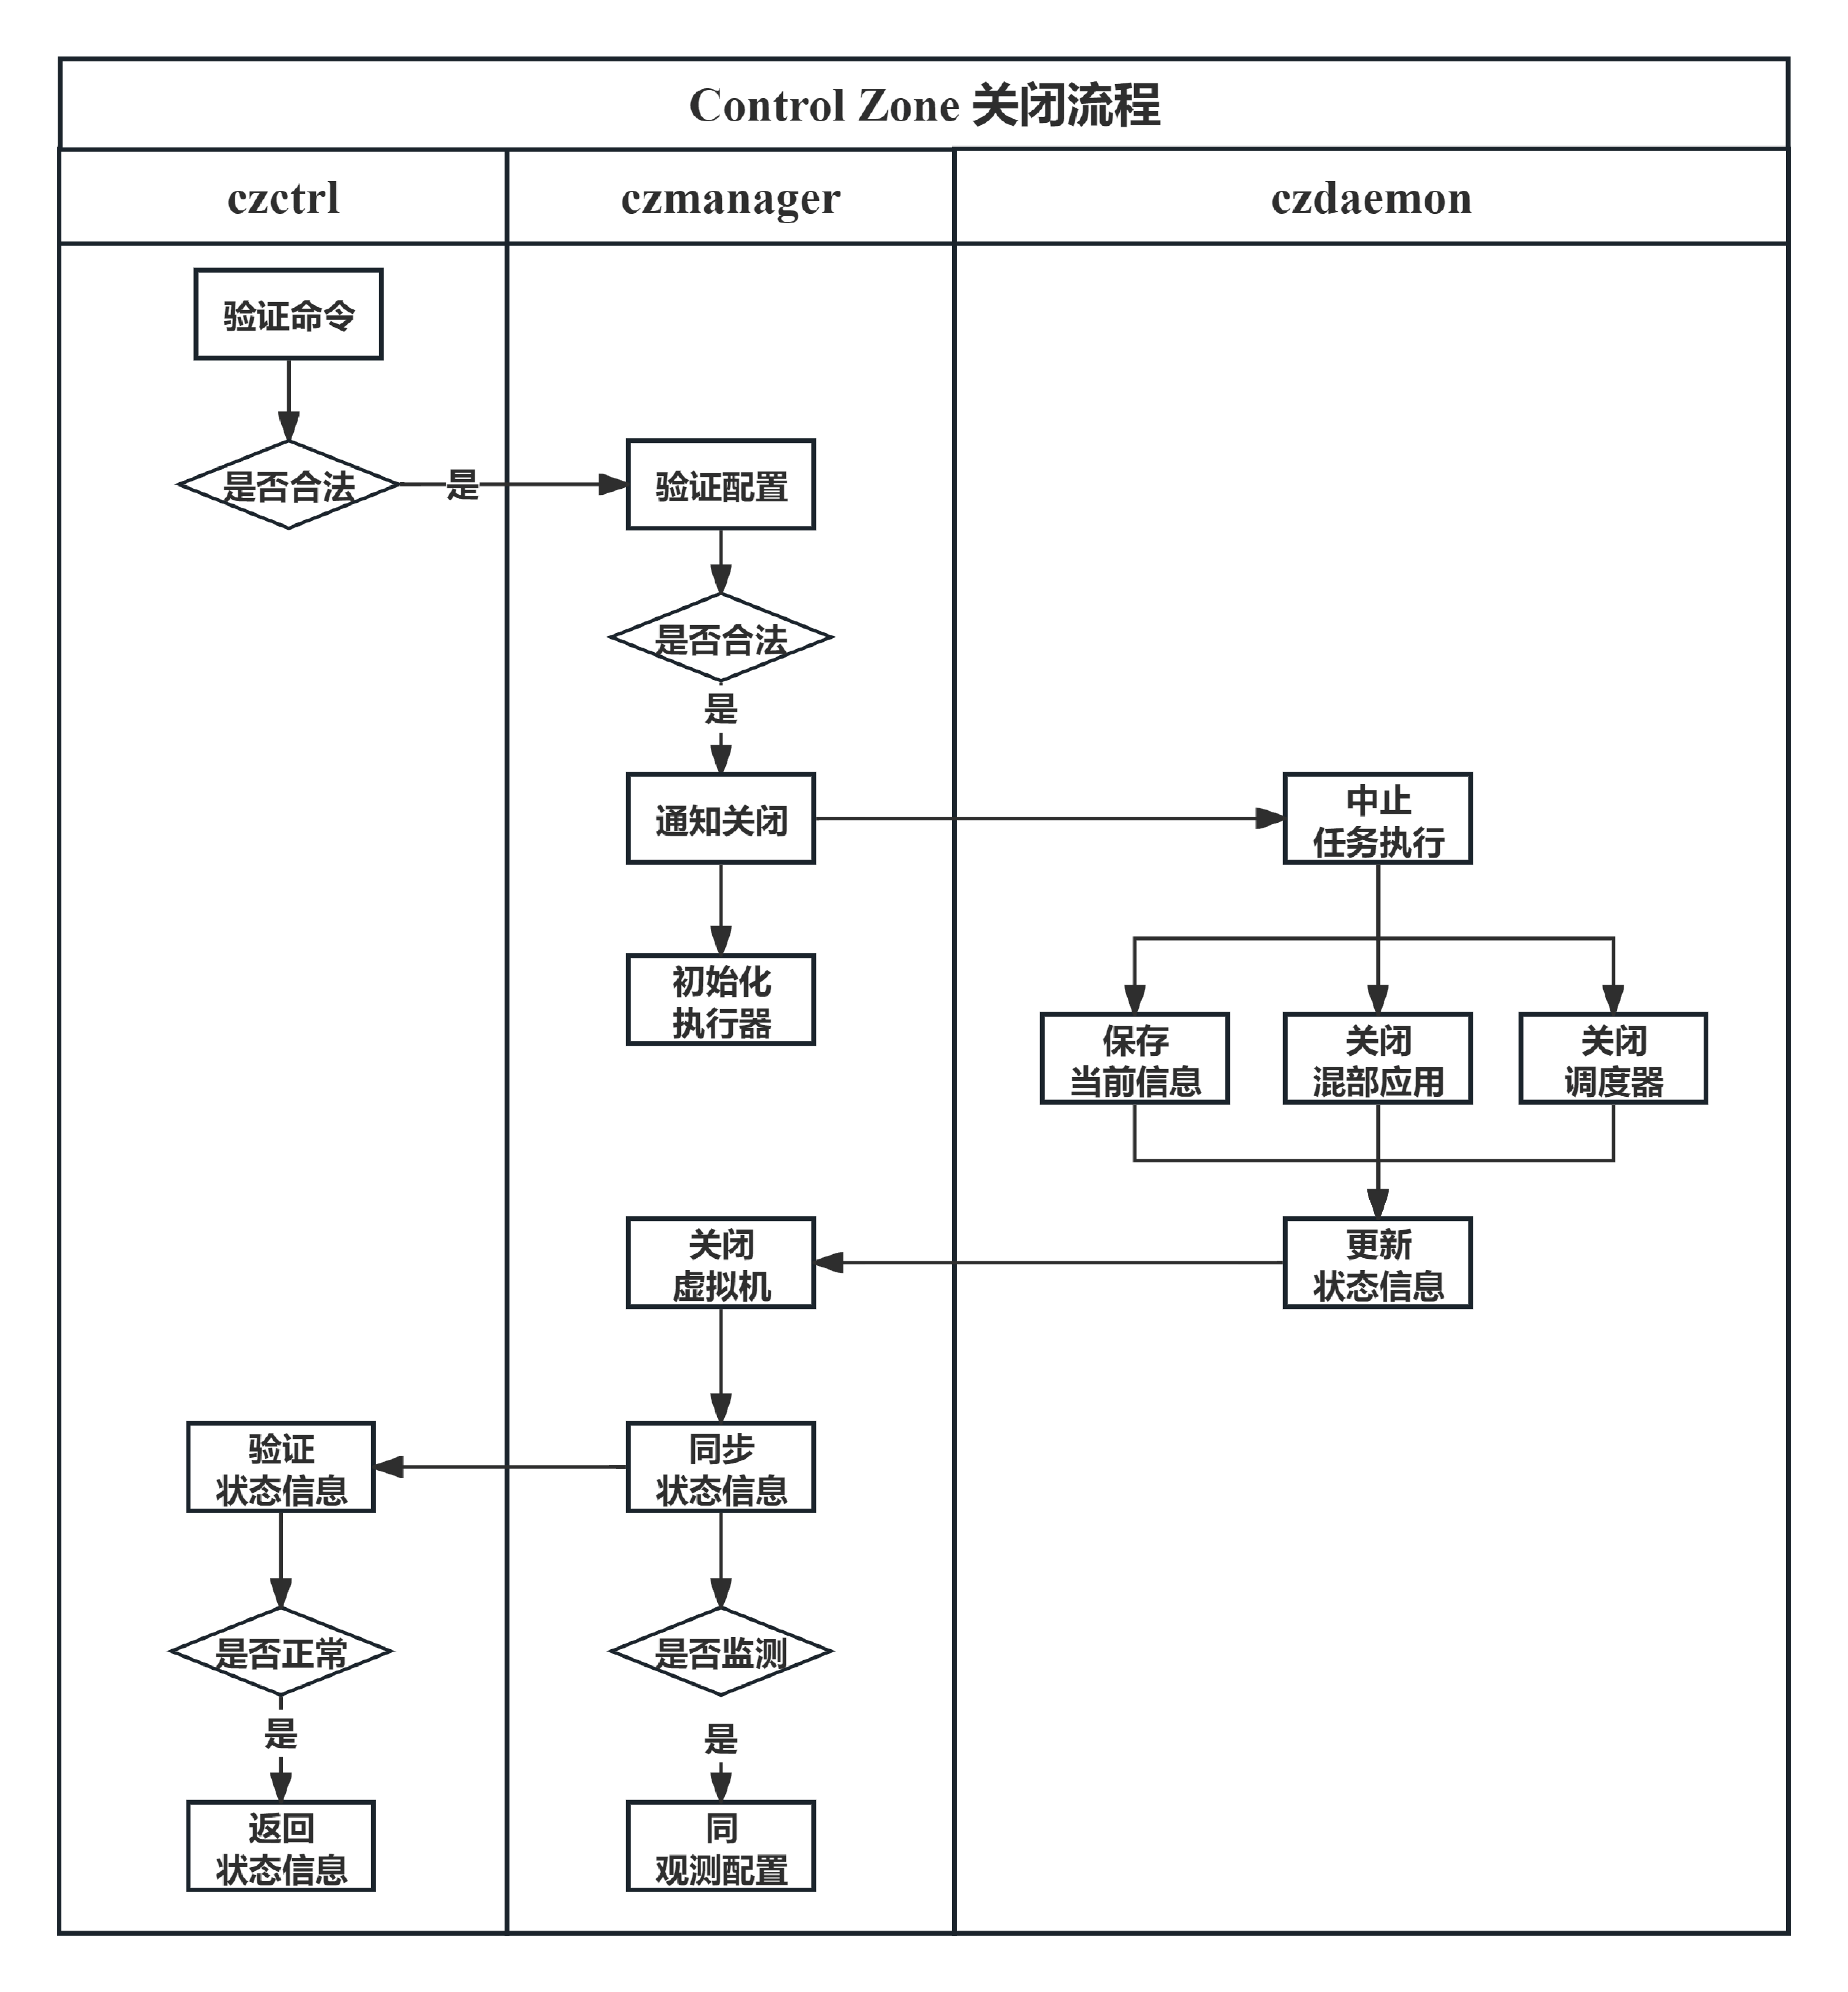
\includegraphics[width=\textwidth]{cz_stop}
        \caption{\quad Control Zone关闭流程}
        \label{fig:cz_stop}
    \end{subfigure}
    \begin{subfigure}[b]{0.53\textwidth}
        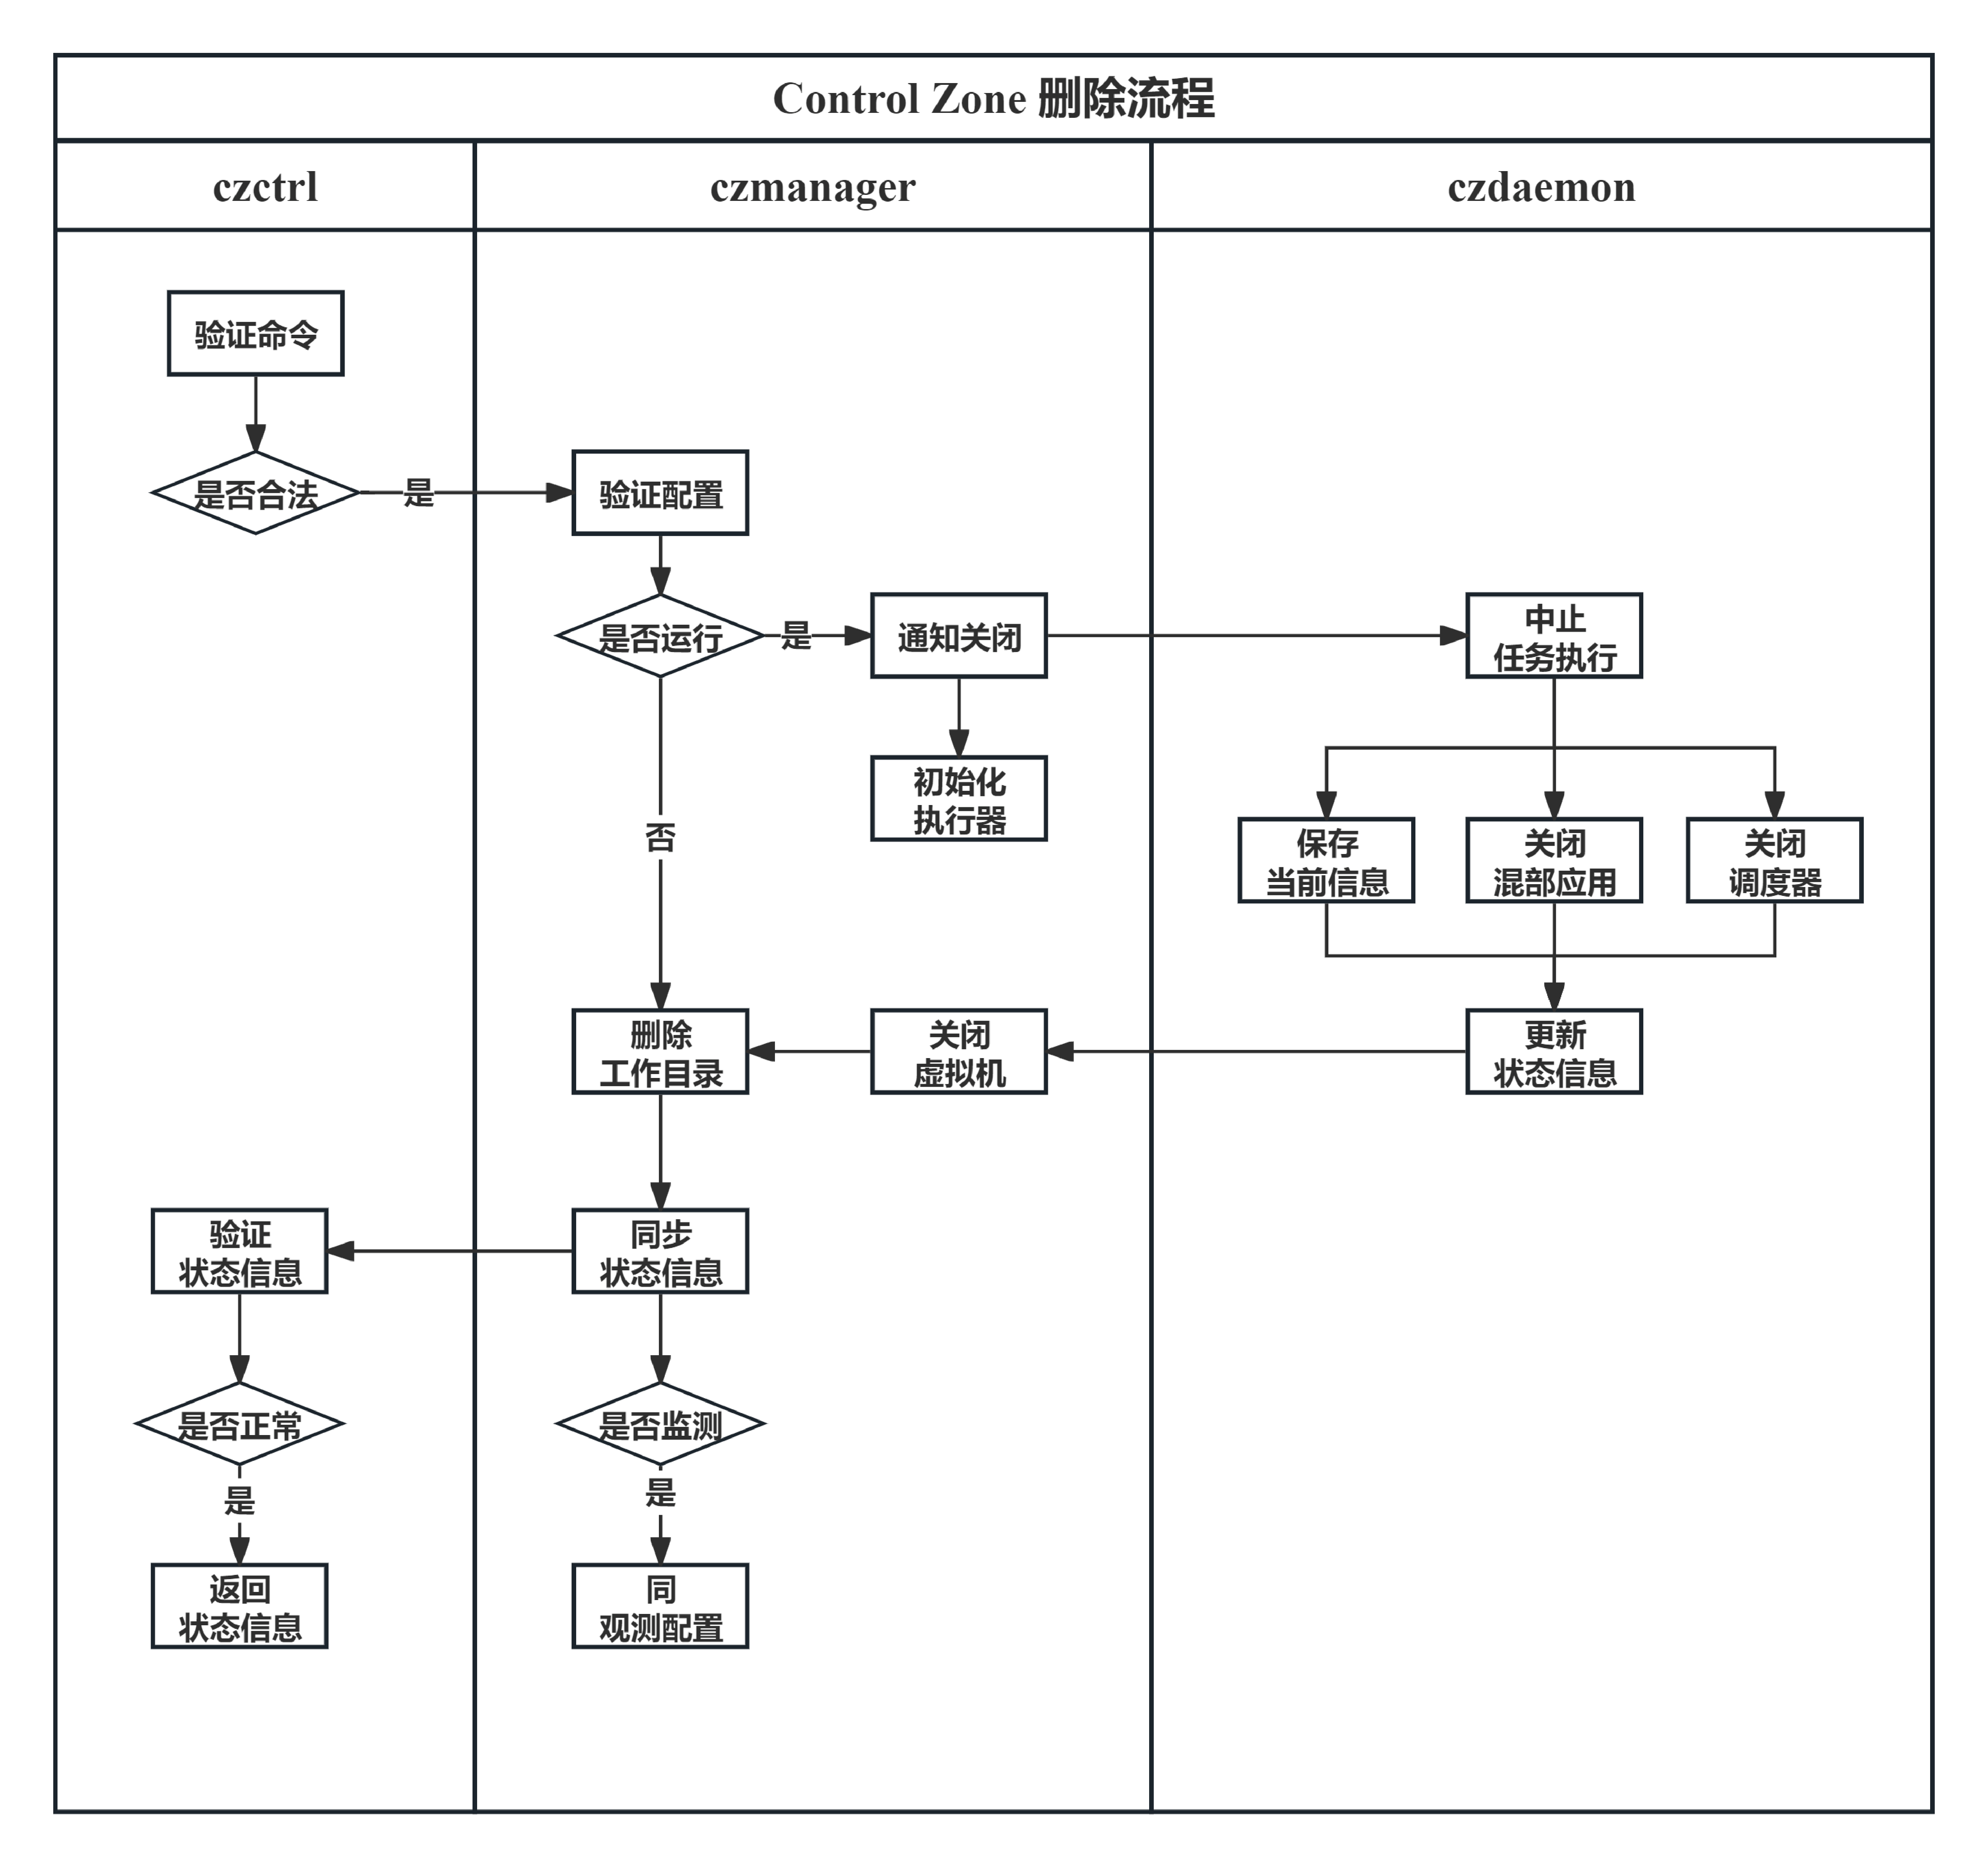
\includegraphics[width=\textwidth]{cz_remove}
        \caption{\quad Control Zone删除流程}
        \label{fig:cz_remove}
    \end{subfigure}
\bicaption{\quad Control Zone关闭与删除流程}{\quad Control Zone closing and deletion process}
\label{fig:cz_create_start}
\end{figure}

Control Zone的删除过程如图~\ref{fig:cz_remove}所示,通常只有已经停止的Control Zone能够被删除,而为简化操作,当Control Zone为其他状态时,此时进行删除操作时会首先将Control Zone的状态转化为停止状态,在进行删除操作。Control Zone的除了工作目录的销毁外,还会回收已经分配的资源。

Control Zone的更新过程如图~\ref{fig:cz_update}所示,Control Zone Yaml中的绝大部分字段都允许被更新,一些字段的更新由czmanager调用资源管理接口完成,如修改cgroup或resctrl等字段中的内容,czmanager发现只有这些字段被修改时,就会重新修改资源隔离配置,并调用各个资源管理接口来进行实施。 而部分字段则会涉及到Control Zone的重新启动,如对Guest中的内核、根文件系统等字段进行修改,czmanager检测到这些字段发生修改后,就会进如重新启动的流程,并在关闭虚拟机之后,实施相关更新内容,再启动虚拟机。更新完毕后,观测配置可能会过时,因此必要时czmanager还会与可观测性基础设施同步观测配置的变化。

\begin{figure}[H]
    \centering
    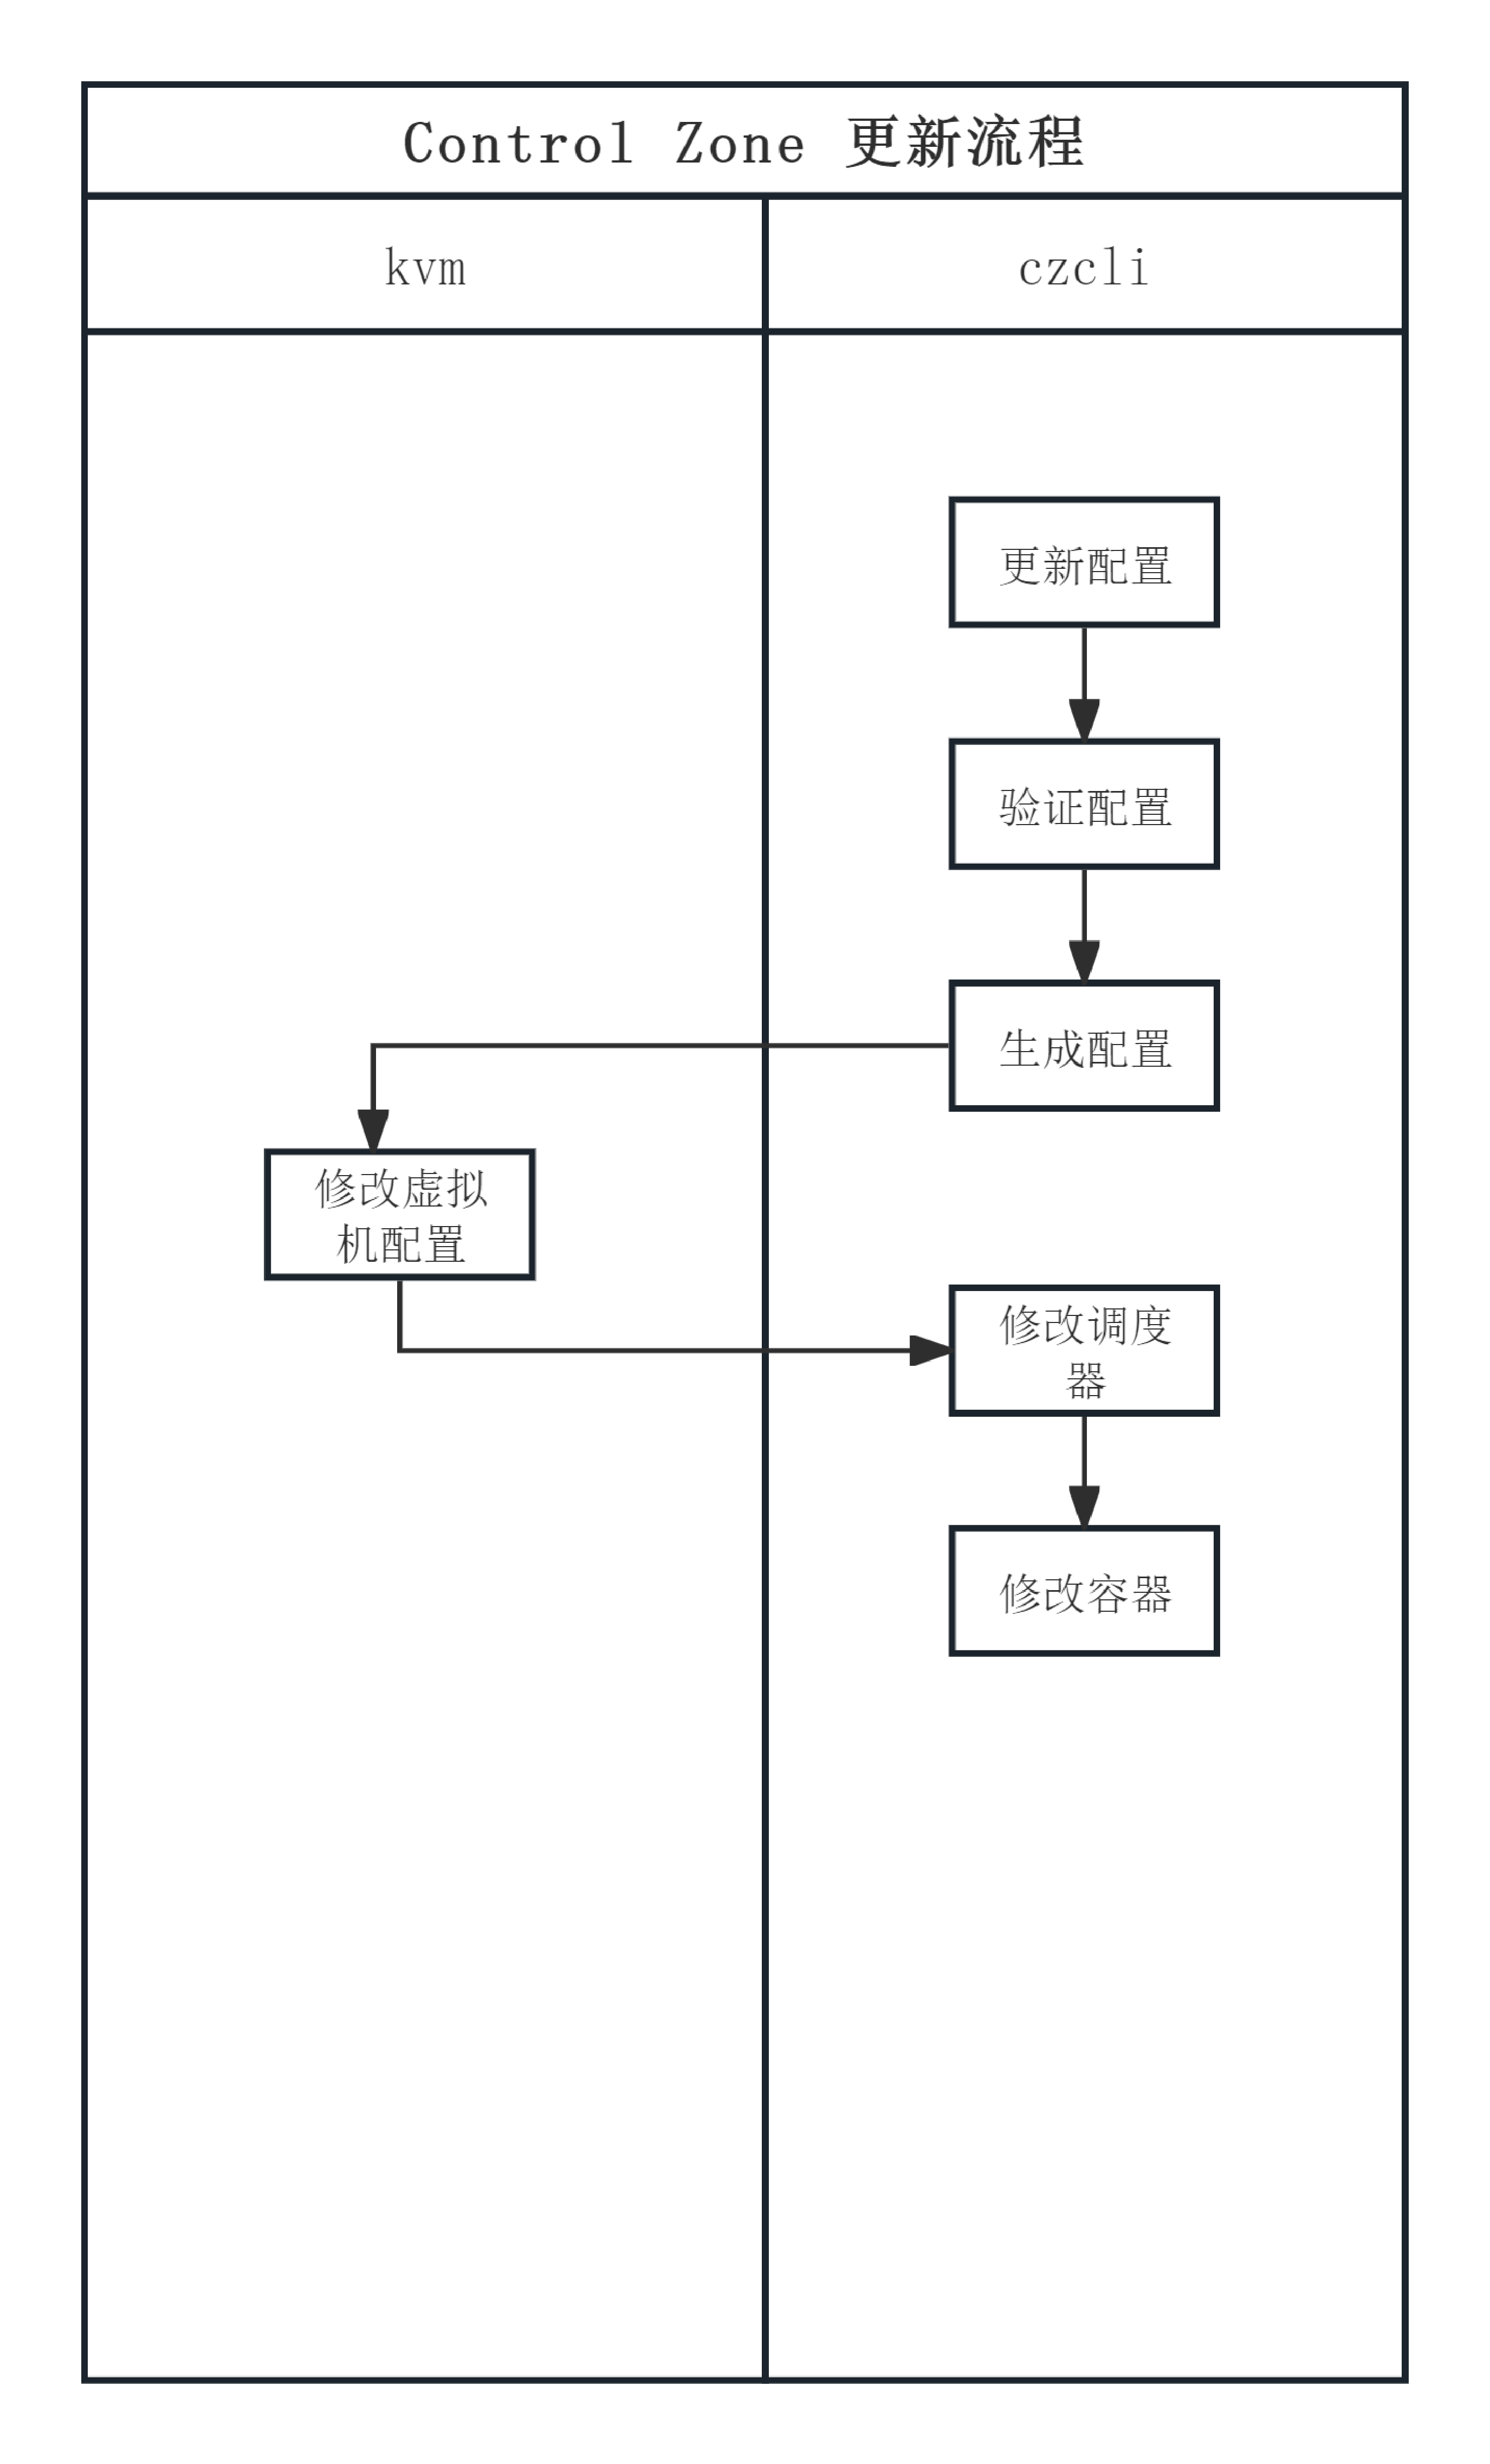
\includegraphics[width=0.7\textwidth]{cz_update}
    \bicaption{\quad Control Zone更新流程}{\quad Stop Control Zone}
    \label{fig:cz_update}
\end{figure}

\subsection{Control Zone开销优化}

% 隔离性实现
% 内核裁切
% hypervisor选择
% 系统功能要求
% 镜像共享

Control Zone中使用虚拟机作为沙箱底座,主要出于隔离性与安全性两个因素的考虑。首先,Control Zone需要一个较强的隔离环境,引入虚拟化一方面增强了隔离效果,同时也能够基于Hypervisor来提供更多的资源限制手段。其次,Control Zone中基于调度子系统来协调多任务的执行,使用虚拟机一方面能够提供场景上的限制,如有限的硬件资源,有限的竞争应用等,其次,修改任务的调度信息是较为风险的行为,如过设置不当有可能引发整个系统的性能劣化,而利用虚拟机能够防止这种风险的扩散。

虚拟机的引入会带来额外的开销,主要体现在虚拟化运行时与系统环境两个层次。一方面,虚拟化运行时需要准备一个完整的虚拟机,而对各个模拟设备进行初始化及配置的过程会产生额外的开销,同时,在虚拟机运行过程中,虚拟化运行时在需要对设备进行模拟,模拟过程中也会产生额外的开销。另一方面,容器中的应用运行之前,还需要经过经过作操作系统、软件环境以及容器运行时三个阶段的运行环境初始化,每个阶段都会产生额外的开销。

沙箱实现中主要从两个方面围绕开销进行优化。首先, 在虚拟化运行时的选择上,沙箱使用CloudHypervisor作为默认的虚拟化运行时,CloudHypervisor与Firecracker类似,都是基于Rust-VMM套件构建的轻量级虚拟化运行时,相比于Firecracker,CloudHypervisor更侧重云场景的实际需求,并额外支持了PCI设备模拟以及PCI设备直通,从而在保证本体轻量的同时,提供更强的性能与更实用的功能\citep{agache2020firecracker}。其次,在系统环境上,沙箱实现时围绕三个阶段进行优化,对于操作系统,沙箱实现时参考了Firecracker Kernel配置,并根据需要增加了对PCI、容器、BPF子系统以及Sched Ext调度类的支持,随后,对于启动过程, 沙箱使能了Linux的PVH(半虚拟化)配置,使得不必经过BIOS就能够直接引导系统,同时,由于Control Zone系统环境足够简单,因此不需要initramfs阶段的引导过程而直接挂载根文件系统进入init初始化过程。然后,对于根文件系统,沙箱使用Alpine\citep{alpine}作为基础镜像,Alpine是一个轻量级Linux发行版,使用Busybox与Musl,其中Busybox是一系列Linux基础工具的集合,只需要一个程序就能够完成Linux中多个程序的功能,同时Busybox代码专注于基础功能并经过了高度简化,通常只会占用极小的存储空间,Musl是一个轻量级的C标准库,其在设计时就专注于提供最基本的C标准函数与特性,因此占用空间较小,同时Musl中优化了一些常见的系统调用,在部分场景下有更好的性能表现。而对于容器运行时,沙箱选择了crun\citep{crun}作为Control Zone中的容器运行时,crun使用C语言开发,相较于使用Go语言开发的runc,crun在启动容器上的开销降低了49.4\%,同时占用的内存也更少。

而为满足多样的使用需求,沙箱也兼容了对Libvirt支持。Libvirt并不是一个虚拟化运行时,而是针对多种虚拟化技术的抽象层,提供了更标准的API来对虚拟机进行管理。通过兼容Libvirt,沙箱能够获取更多的特性,尤其在可观测性上,沙箱能够借助Libvirt提供的丰富监控机制,从而更方便地为可观测性基础设施提供监测数据。

% \subsection{资源隔离技术}
% - cgroup
% - resctrl / intel RDT
% - hpv virt device

\section{实验设计与分析}

\subsection{实验环境}

实验环境有两台服务器构成,服务器硬件信息如表~\ref{tab:exp_env}所示。在CPU资源上,每台服务器上包含有两个Socket,单台总计80个物理核心,划分为4个Numa Node,同时,CPU均开启超线程,并使能Intel RDT,从而为可观测性基础设施提供末级缓存及内存带宽的监控,并为虚拟机提供按路数的末级缓存划分和固定补偿的内存带宽调控功能。在网络资源上,服务网卡支持SRIOV技术,能够为有网络性能需求的虚拟机提供硬件直通服务。

\begin{table}[H]
    \bicaption{\quad 服务器硬件参数}{\quad Server Hardware Information}% caption
    \label{tab:exp_env}
    \footnotesize% fontsize
    \setlength{\tabcolsep}{4pt}% column separation
    \renewcommand{\arraystretch}{1.25}% row space 
    \centering
    \begin{tabular}{lc}
        \hline
        硬件资源 & 硬件信息 \\
        \hline
        CPU & Intel Xeon Gold 6148 (40 cores) * 2 \\
        Processor Core Frequency & 2.4GHz,Turbo 3.7 GHz \\
        L1 Caches & 32KB,  8-way set associative, split D/I \\
        L2 Caches & 1024KB, 16-way set associative \\
        L3 Caches & 28160KB, 11-way set associative \\
        Main Memory & 32GB * 8, 2666MHz DDR4 \\
        NIC & Intel Corporation Ethernet Connection X722 for 10GbE SFP+(10Gbit) \\
        \hline
    \end{tabular}
\end{table}

每台服务器的系统软件环境如表~\ref{tab:system_env}所示。在操作系统上,实验中选择使用较常见的Ubuntu22.04 LTS,Ubuntu同时也是Sched Ext优先支持的发行版,能够较方便地通过包管理工具安装预编译的Sched Ext内核。在虚拟换运行时上,Qemu采用发行版所支持的稳定版,而以轻量为目标的CloudHyeprvirsor则采用自编译的最新发布版本。

\begin{table}[H]
    \bicaption{\quad 服务器系统环境}{\quad Server System Information}% caption
    \label{tab:system_env}
    \footnotesize% fontsize
    \setlength{\tabcolsep}{30pt}% column separation
    \renewcommand{\arraystretch}{1.25}% row space 
    \centering
    \begin{tabular}{lc}
        \hline
        软件类型 & 软件信息 \\
        \hline
        系统 & Ubuntu 22.04.3 LTS  \\
        内核 & 5.15.0-79-generic \\
        虚拟化运行时 & cloud-hypervisor v38.0-150 \\
                   & QEMU emulator version 6.2.0 \\
        其他        & libvirtd 8.0.0 \\
        \hline
    \end{tabular}
\end{table}

除系统软件之外,每台服务器还按照需要部署了其他关键服务。其中可观察基础设施按照第三章中所论述的架构进行搭建,Master节点上部署的了Prometheus与Grafana,用于进行数据采集与离线分析,Node节点上则部署的第三章中所提到的一系列Exporter,提供各个维度数据的采集能力。Master除对数据进行采集、存储、分析外,还额外部署了Harbor来对外提供容器管理服务,并承担大部分的配置文件存储。Node作为主要的实验场地,安装了Control Zone沙箱的所有相关的组件,并承担主要的服务运行。实验中对于Client-Server类型的任务,为尽可能地模拟真实环境,因此一般将Client放置在Master上。最后,实验中所涉及的关键服务都以容器镜像的形式分发并运行,因此在每个服务器上都需要安装容器运行时,而在容器运行时的选择上,对性能不敏感而对稳定性有要求的Master上使用Docker来提供容器服务,而在Node上,则使用Podman作为容器运行时,Podman相较Docker更加轻量,同时不存在Docker、Containerd等后台驻留服务,能够提供较为纯净的容器运行环境。

\subsection{启动开销实验}

Control Zone的启动开销计算从虚拟化运行时开始到系统引导至init过程的时间,虚拟机使用1CPU与512M内存的基础配置,在虚拟化运行时上,选择CloudHyperviosr与Qemu进行对比,而在精简内核上,选择Alpine Virt内核、Control Zone内核,以及CloudHyeprvirsor、Firecracker的默认精简内核,其中Alpine Virt内核为社区提供给云厂商的标准虚拟机内核,启动了大部分Guest优化功能,但同时也保留了对于众多设备的支持,而以轻量为目标的CloudHyeprvirsor、Firecracker也各自提供了默认的精简内核,相较于Alpine Virt内核,去除了大量无意义的驱动,几乎只支持virtio设备,其中CloudHypervisor默认内核还额外使能了PCI子系统,以便于使用SRIOV设备,实验中为了让实验结果更加具备可比性,因此使能了Firecracker内核中的PCI配置。

\begin{figure}[H]
    \centering
    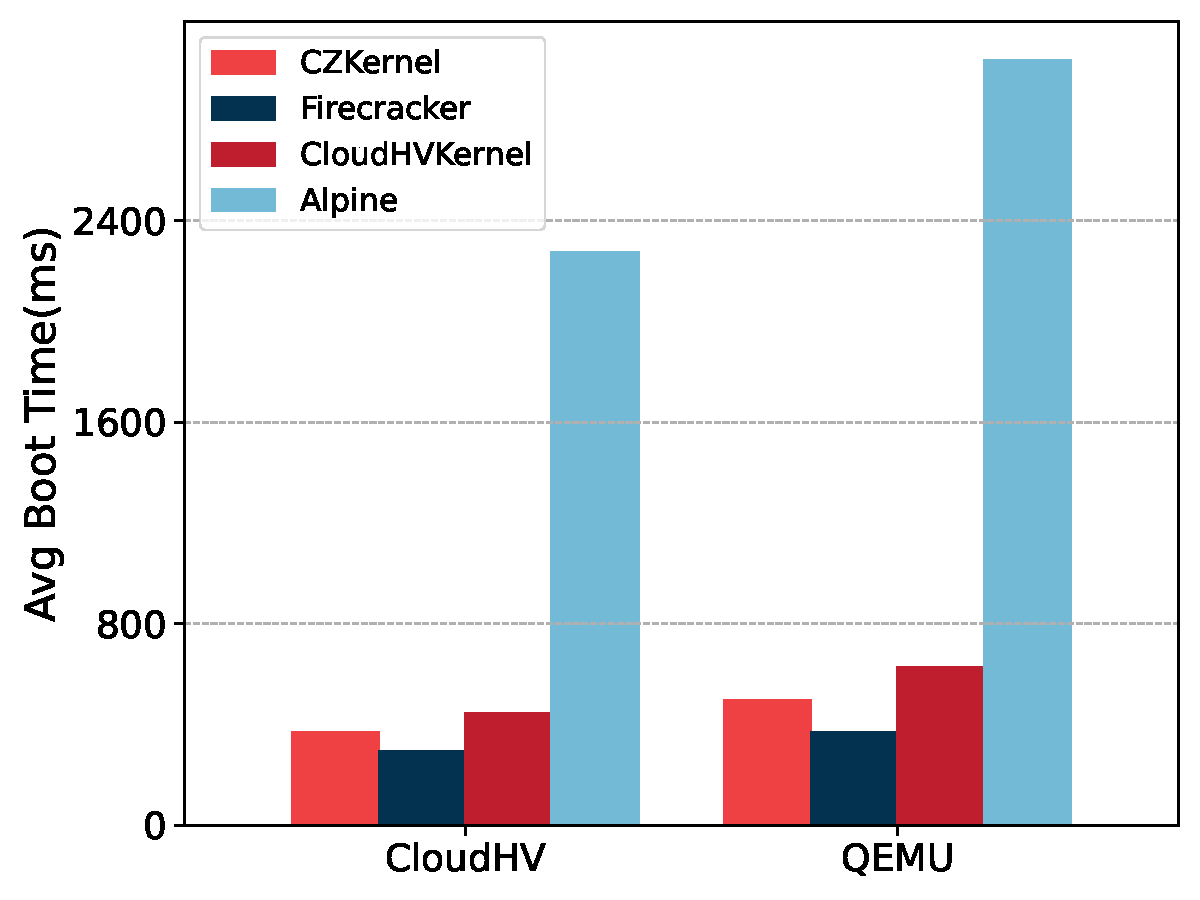
\includegraphics[width=0.55\textwidth]{avg_boot_time}
    \bicaption{\quad 平均启动时间比较}{\quad Comparison of average boot times}
    \label{fig:avg_boot_time}
\end{figure}

实验结果如图~\ref{fig:avg_boot_time}所示,Control Zone内核的平均启动开销相较于Alpine Virt内核最高降低了88.8\%,对比不同的虚拟化运行时的数据发现而其中绝大部分的优化效果升来自于对内核的裁切,Control Zone内核仅支持运行容器、BPF子系统与Sched Ext调度类的最小功能,因此在启动时省去了大量非必要的工作,从而能够做到足够快速。同时还可以发现, 对于Alpine Virt内核而言,使用CloudHypervisor相较于Qemu降低28.9\%的启动时间,而观察两者的启动日志发现,虚拟化运行时所带来的提升主要来自于对于设备的裁切上,CloudHypervisor只需要针对云场景,因此相较于Qemu去除了大量的无关设备模拟,而更精简的设备一方面减少了虚拟化运行时的启动时间,另一方面,Guest内核也不必进行过多的设备探测与初始化,尤其在PCI子系统的初始化上,CloudHypervisor相较于Qemu,PCI子系统的初始化时间平均减少了83.2\%。相同的情况在其他内核上则有所不同,由于精简内核本身支持的设备驱动就十分有限,因此虚拟化运行时在这些内核的优化上主要体现在运行时启动本身上。

\begin{figure}[!htbp]
    \centering
    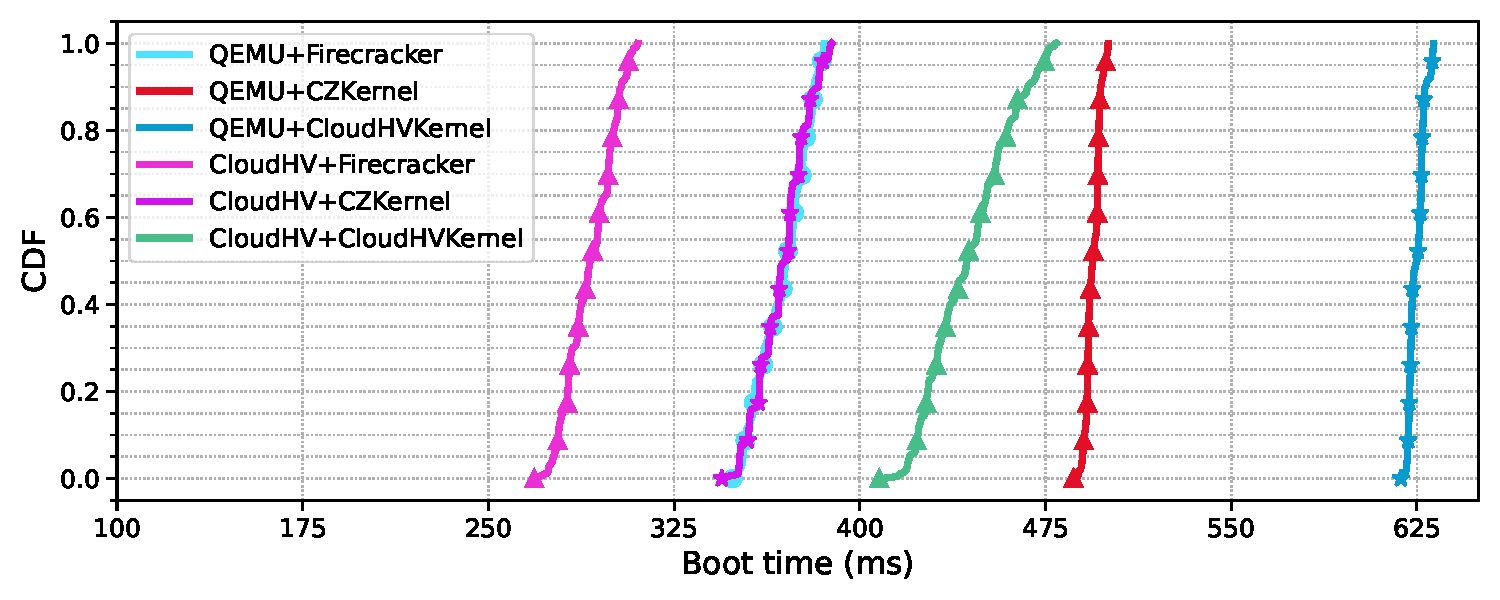
\includegraphics[width=0.8\textwidth]{boot_time_cdf}
    \bicaption{\quad 精简内核的启动时间比较}{\quad Comparison of Kernel Boot Time Optimization} 
    \label{fig:boot_time_cdf}
\end{figure}

在精简内核的对比中,Control Zone内核也存在优势,如图~\ref{fig:boot_time_cdf}所示,使用Qemu时,Control Zone内核相较于CloudHypervisor默认内核在启动时间上减少了20.6\%,对比两者配置差异发现,CloudHypervisor所提供的精简内核虽然去掉了大部的驱动支持,但仍然保留了对嵌套虚拟化的支持而开启了虚拟化子系统,因此会产生额外的开销,而Control Zone内核所支持的容器环境所需要的支持则相对更少。但是相对于Firecra内核,Control Zone内核则在启动开销上并没有优势,即便使用Qemu虚拟化运行时,Firecracker内核也能达到接近使用CloudHypervisor的Control Zone内核的启动速度,比较配置能够发现, Firecracker内核在功能裁切上更加激进,分析两者的启动日志能够发现这开销的差异主要来自于Control Zone内核中所需要的额外功能,如Netfilter子系统等。这些功能在本设计中时必须的,同时考虑场景上的差异,Firecracker实现时希望以承担安全容器的运行时环境,虚拟机的生命周期与运行在其中的容器绑定,而在Control Zone的设计中,任务与Control Zone并非完全耦合,Control Zone更接近与对于隔离环境的声明,在任务需要运行时启动,而在任务运行完毕后仍然会保留,并提供给下一个任务使用,即Control Zone不会频繁地启动,因此这部分开销在设计中是可以接受的。

\subsection{性能开销实验}

而为测试实际应用上的性能开销,实验中选择典型应用分析中的6种应用进行性能测试。在内核性能上,选择与CloudHypervisor默认Linux内核进行比较,并同时运行在Control Zone沙箱上。而在沙箱性能上,选择与在Host上以容器的形式部署的应用进行比较。

性能开销实验结果如图~\ref{fig:perf_app}所示,总体来看,Control Zone在内核性能上优于CloudHypervisor默认的Linux内核,而在沙箱性能上,Control Zone也能够在一些应用上取得比Host更好的效果。

\begin{figure}[!htbp]
    \centering
    \begin{subfigure}[b]{0.32\textwidth}
        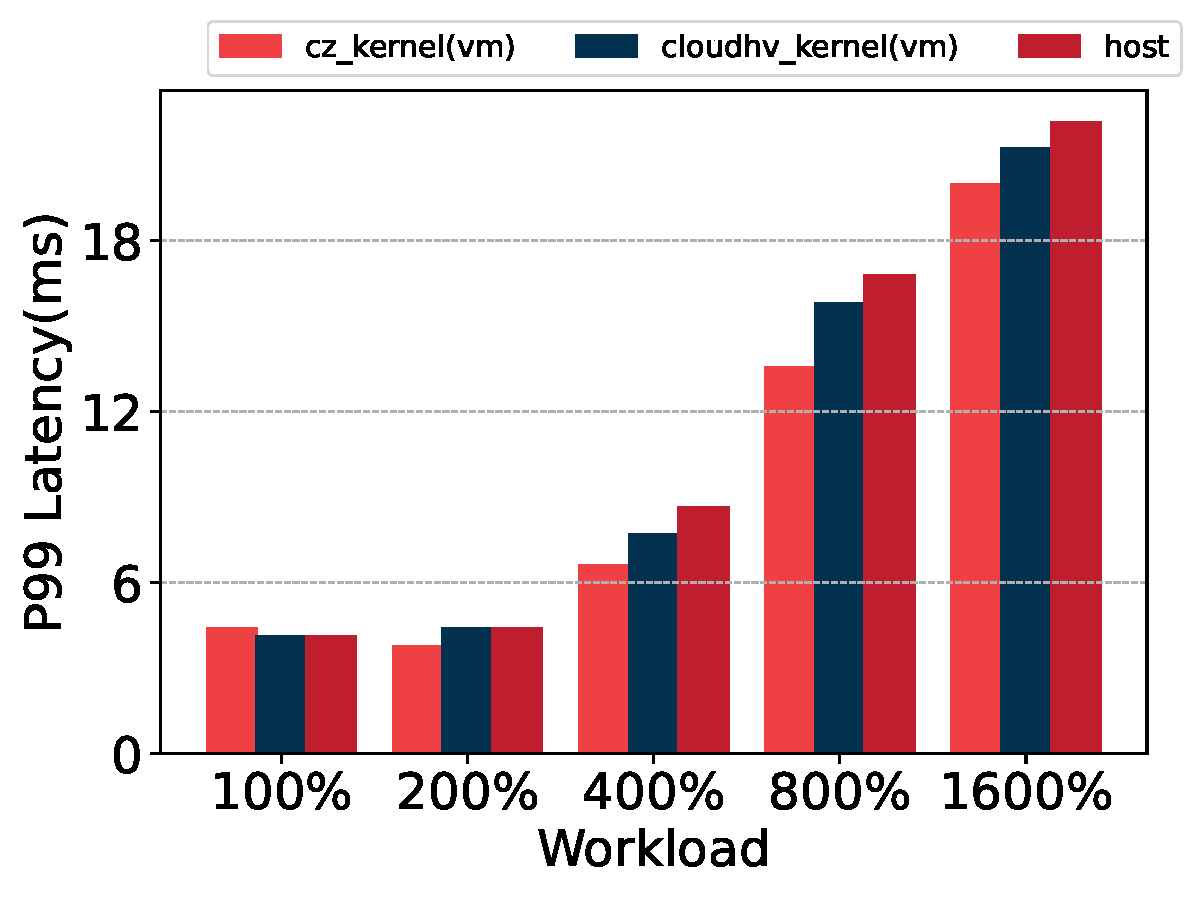
\includegraphics[width=\textwidth]{perf_redis}
        \caption{\quad Redis延迟}
        \label{fig:perf_redis}
    \end{subfigure}
    \begin{subfigure}[b]{0.32\textwidth}
        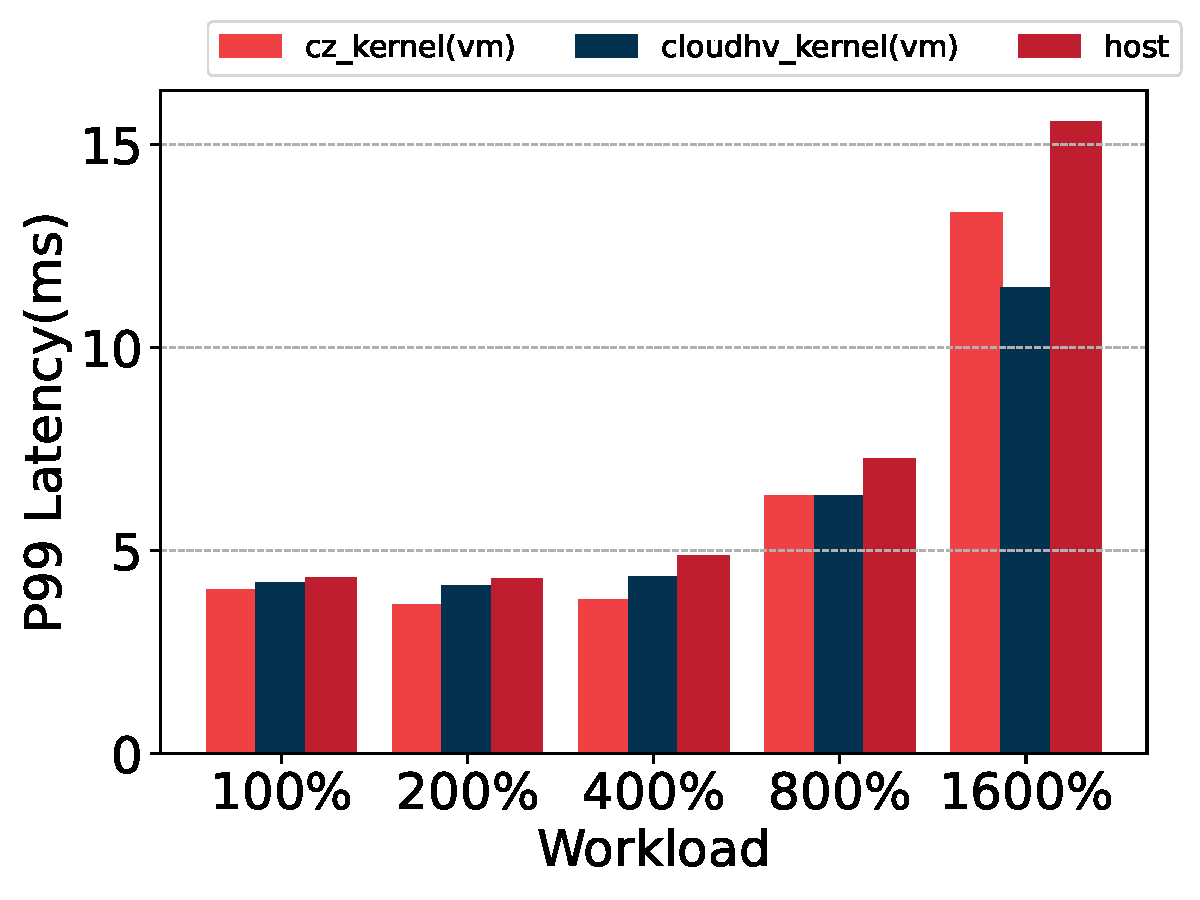
\includegraphics[width=\textwidth]{perf_memcached}
        \caption{\quad Memcached延迟}
        \label{fig:perf_memcached}
    \end{subfigure}
    \begin{subfigure}[b]{0.32\textwidth}
        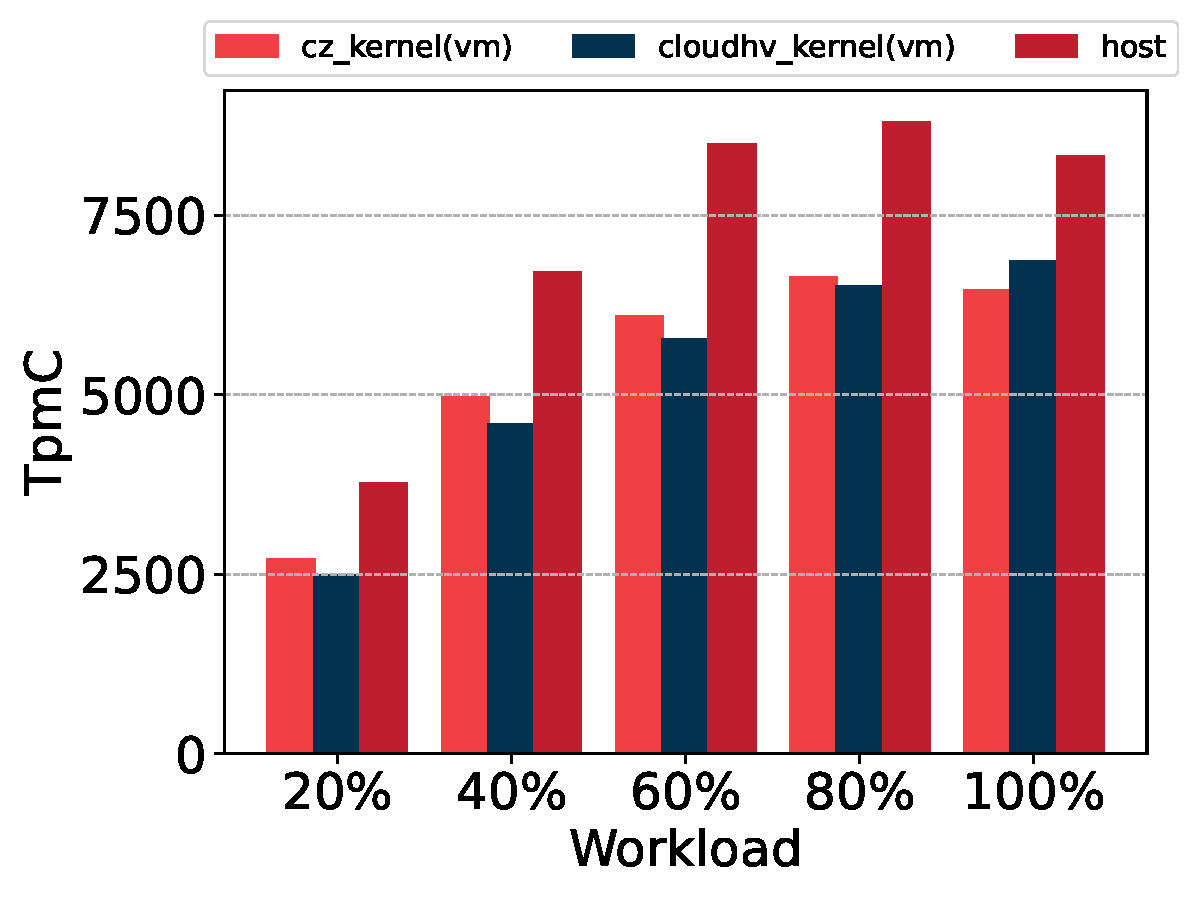
\includegraphics[width=\textwidth]{perf_mysql}
        \caption{\quad MySQL每秒事务}
        \label{fig:perf_mysql}
    \end{subfigure}
    \begin{subfigure}[b]{0.32\textwidth}
        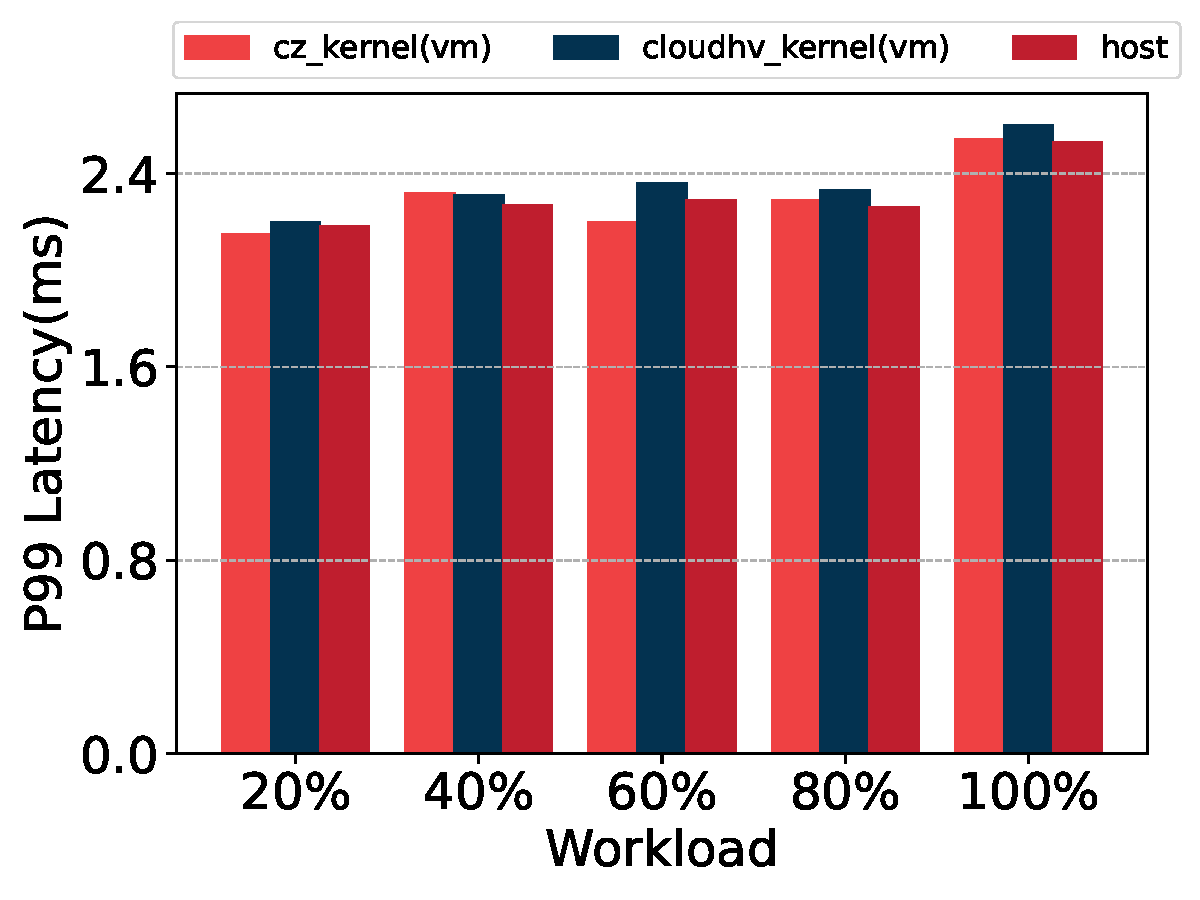
\includegraphics[width=\textwidth]{perf_nginx}
        \caption{\quad Nginx延迟}
        \label{fig:perf_nginx}
    \end{subfigure}
    \begin{subfigure}[b]{0.32\textwidth}
        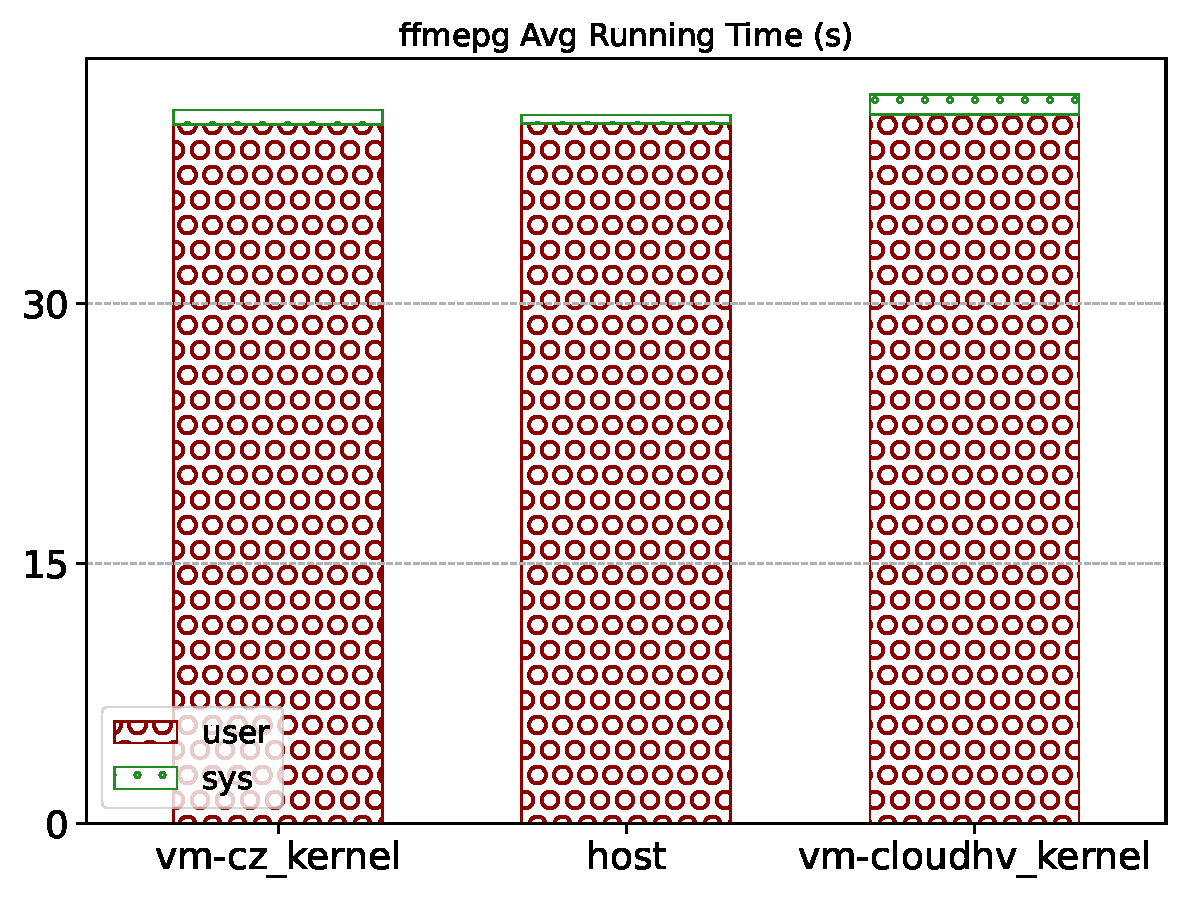
\includegraphics[width=\textwidth]{perf_ffmpeg}
        \caption{\quad FFmpeg运行时间}
        \label{fig:perf_ffmpeg}
    \end{subfigure}
    \begin{subfigure}[b]{0.32\textwidth}
        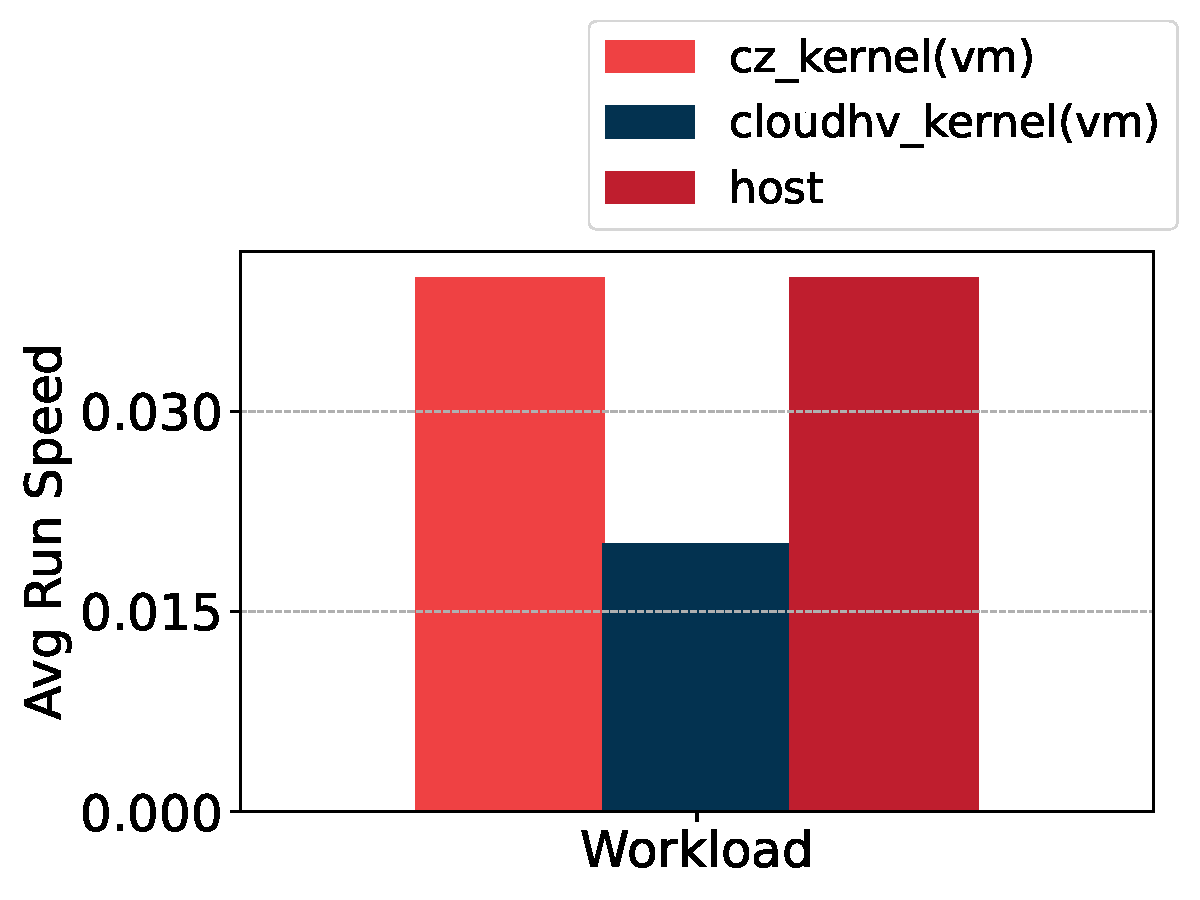
\includegraphics[width=\textwidth]{perf_graph500}
        \caption{\quad Graph500运行时间}
        \label{fig:perf_graph500}
    \end{subfigure}
\bicaption{\quad 应用性能比较}{\quad Application performance comparison}
\label{fig:perf_app}
\end{figure}

Control Zone内核仅以提供隔离的内核环境为目标,在此目标上进行的内核配置裁切能够更加积极。相较于CloudHypervisor默认内核,Control Zone内核在同样仅支持Virtio设备的同时,裁切了如Netfilter等在沙箱中不必的内核功能,从而进一步减少内核中如网络处理路径的长度。在网络应用延迟上,与同样运行在虚拟机中的CloudHypervisor内核相比,Control Zone实现了99分位尾延迟降低最高15.7\%的效果。同时,与直接运行在Host上相比,Control Zone即便引入了虚拟化开销,也能够实现99分尾延迟降低最高38.5\%的效果。但是,对于一些逻辑复杂的应用,如MySQL,则存在一定的性能劣化,主要原因是虚拟设备的性能限制。而在当前虚拟化技术中,通过SRIOV等硬件直通手段能够有效地处理这一问题。

\subsection{性能保障实验}

\begin{figure}[H]
    \centering
    \begin{subfigure}[b]{0.49\textwidth}
        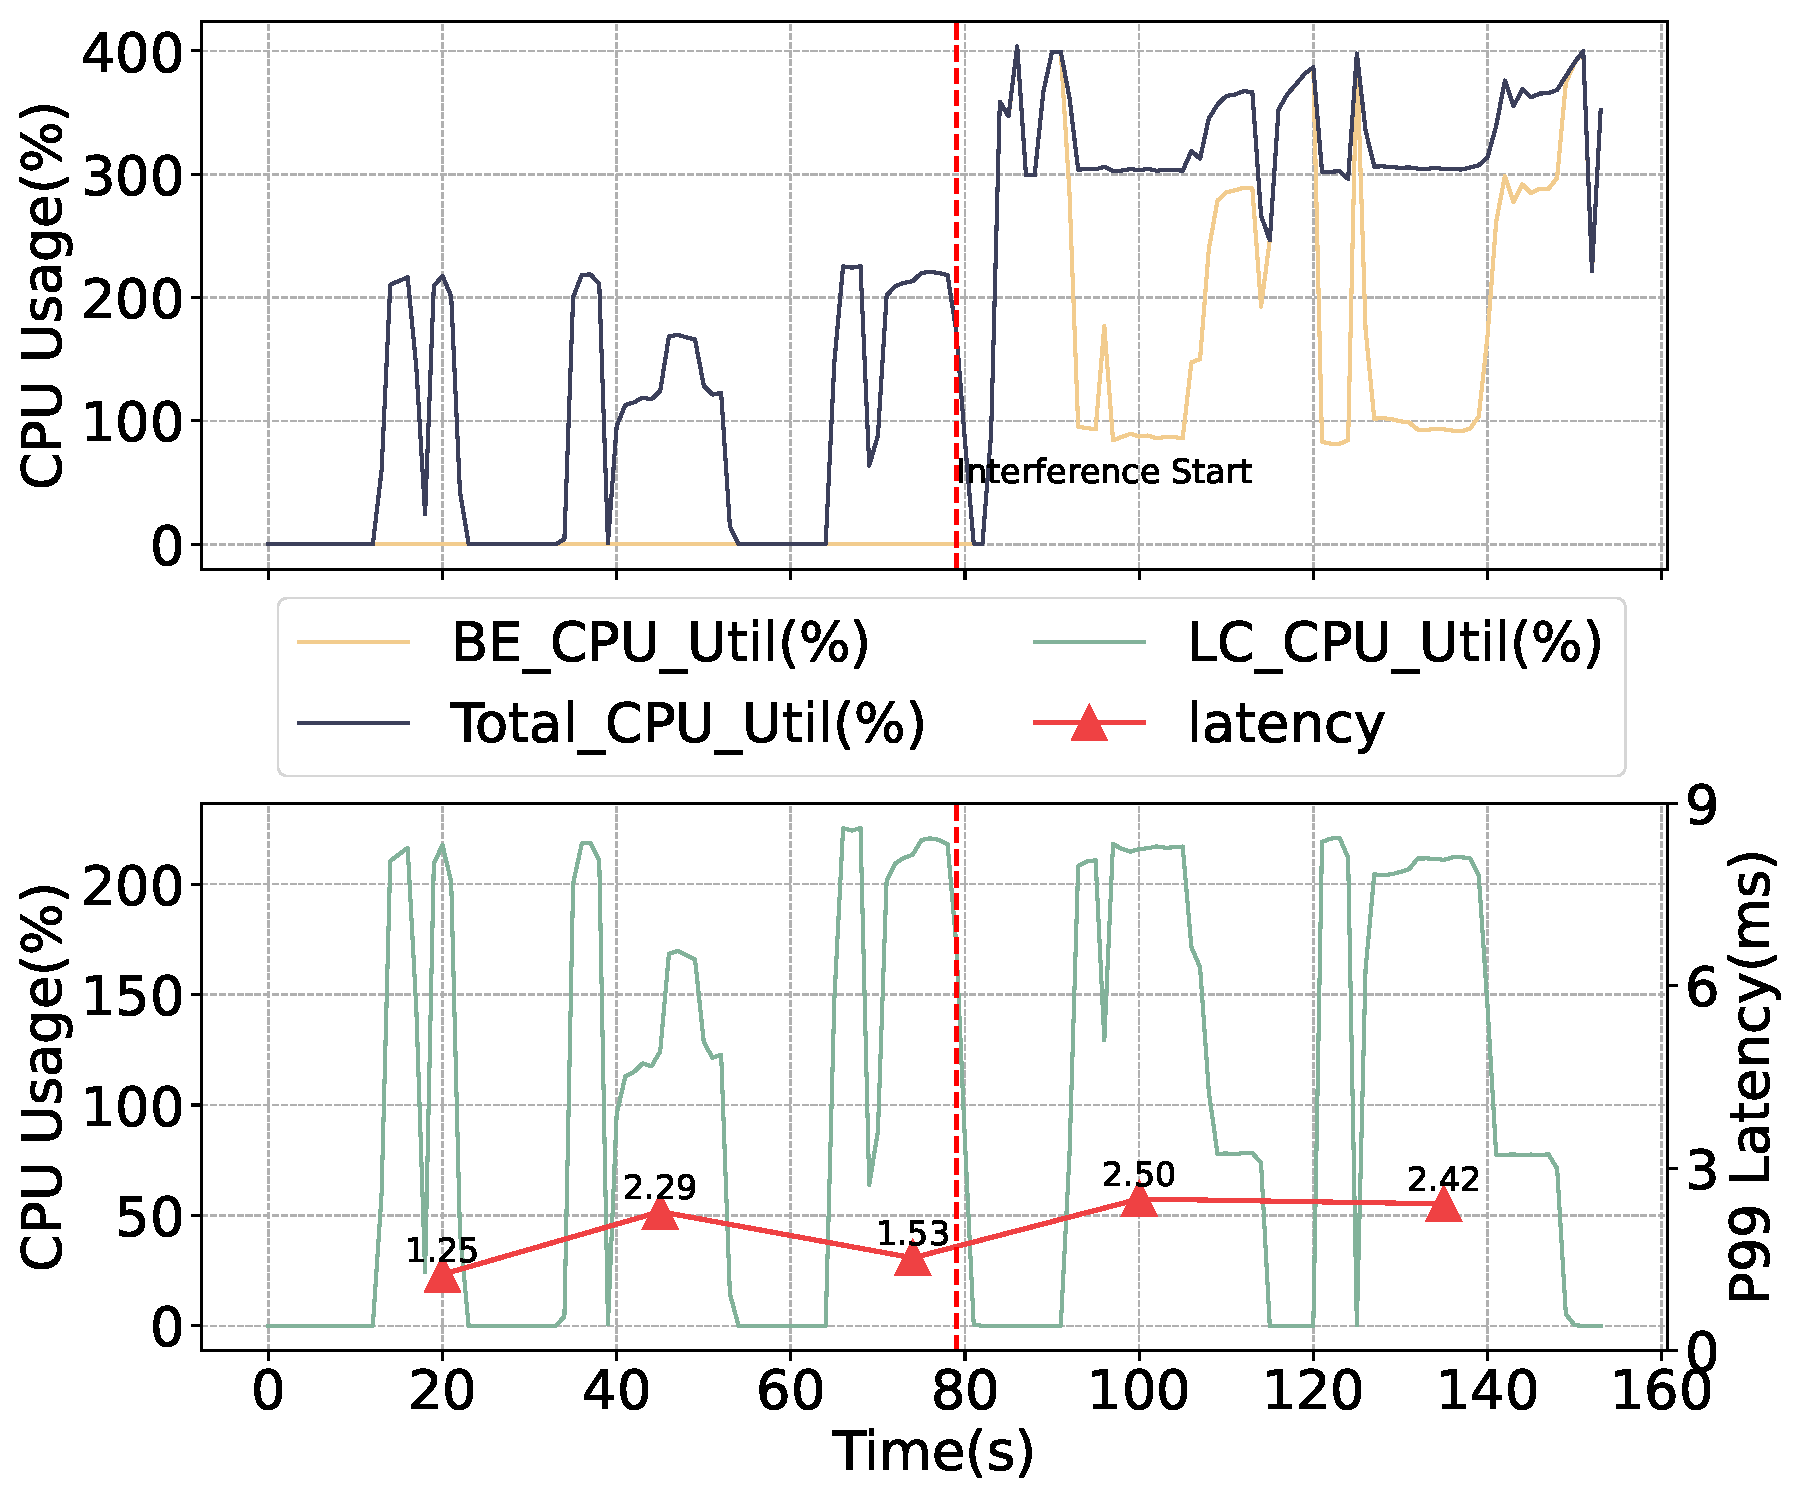
\includegraphics[width=\textwidth]{cpu_series_memcached_ct}
        \caption{\quad Control Zone性能保障}
        \label{fig:cpu_series_memcached_ct}
    \end{subfigure}
    \begin{subfigure}[b]{0.49\textwidth}
        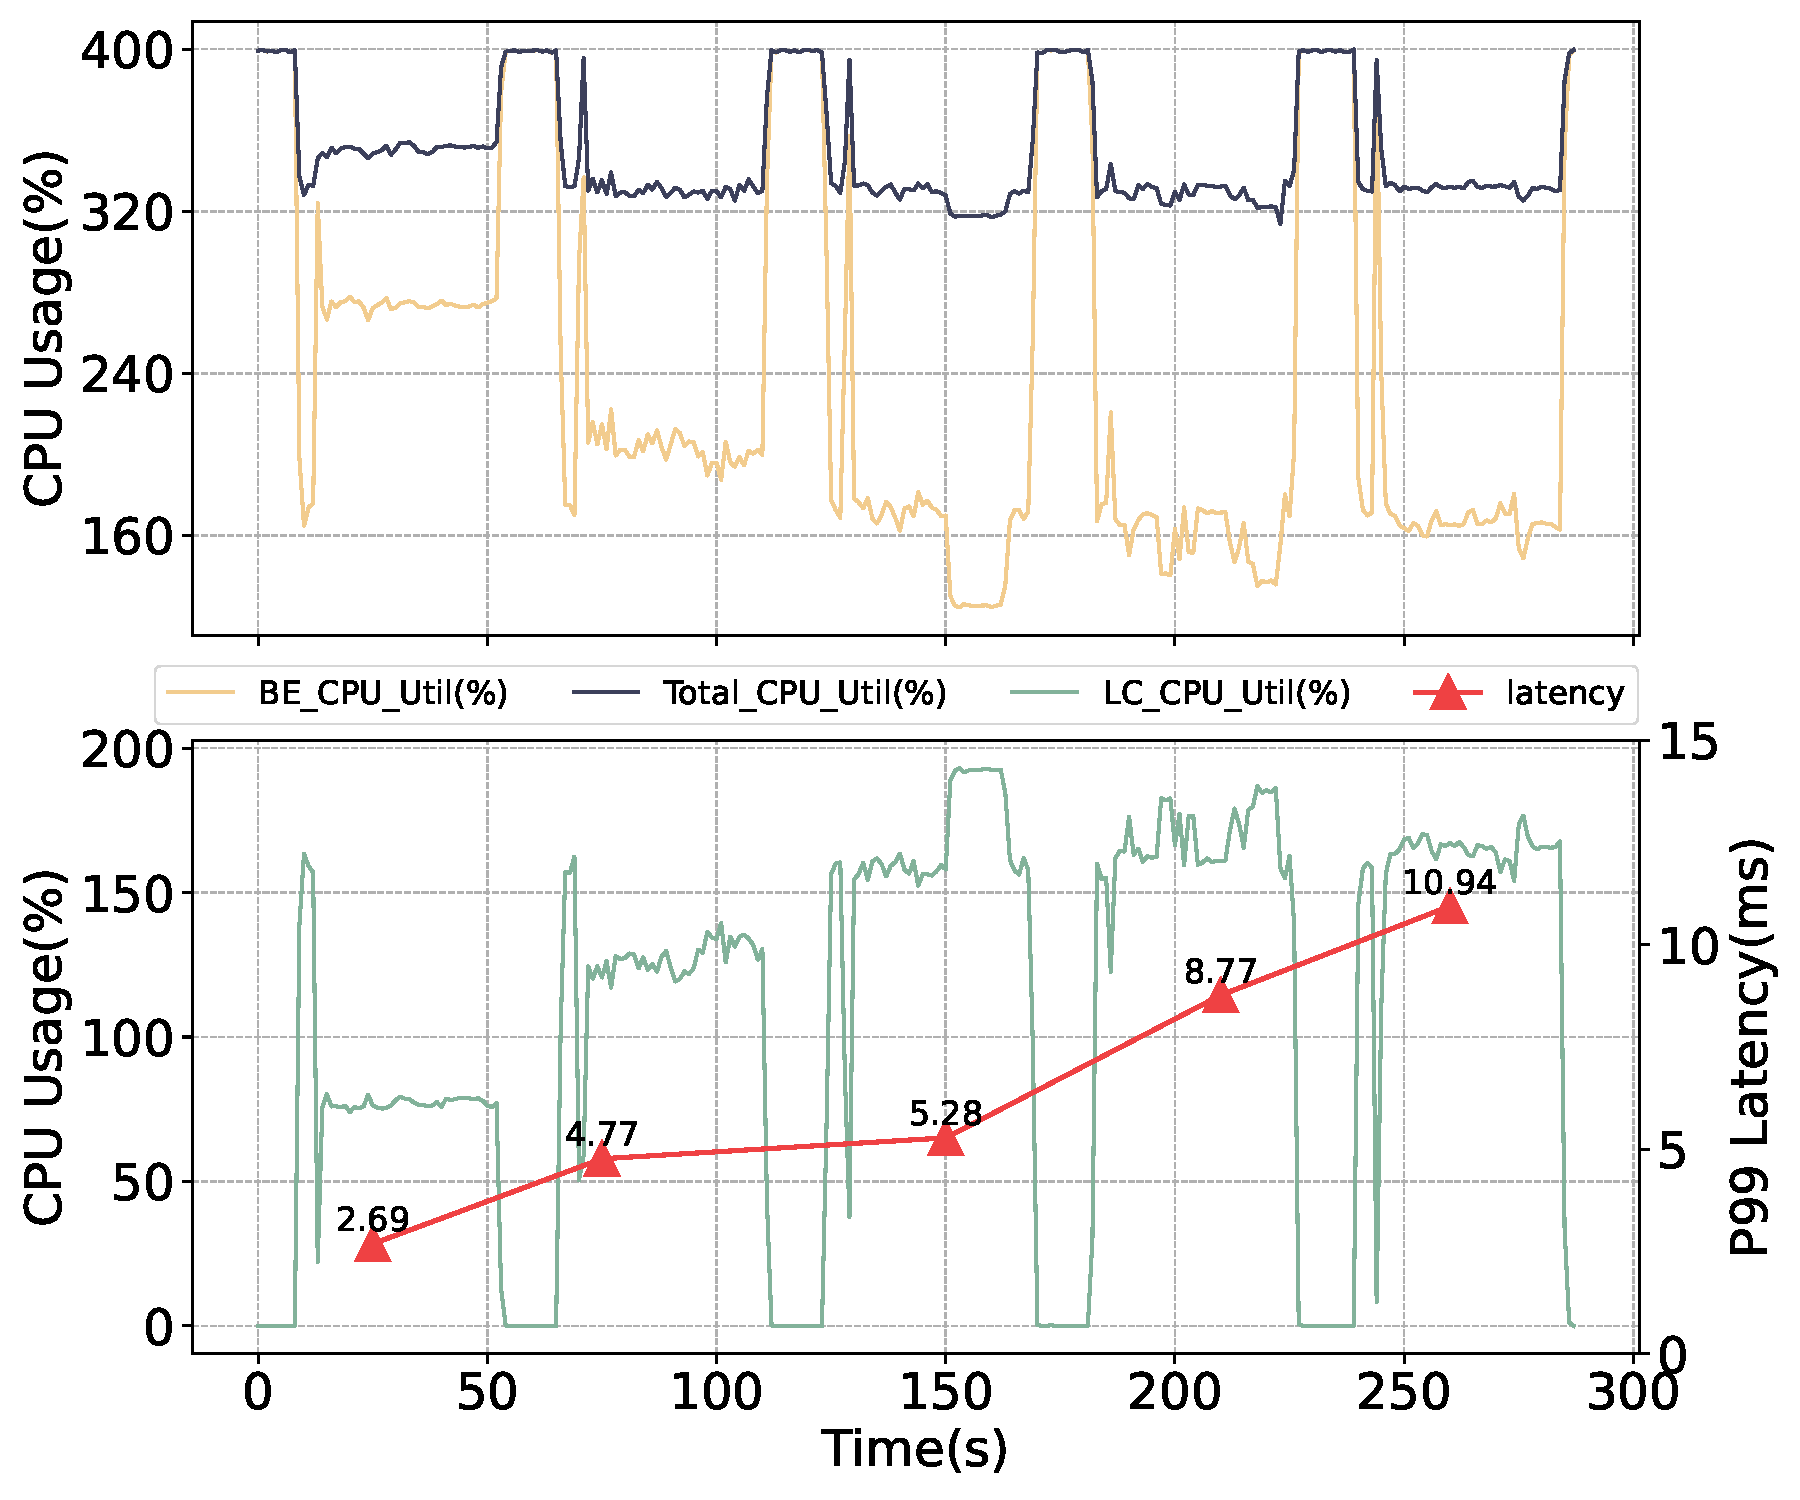
\includegraphics[width=\textwidth]{cpu_series_memcached_eevdf}
        \caption{\quad EEVDF性能保障}
        \label{fig:cpu_series_memcached_eevdf}
    \end{subfigure}
    \bicaption{\quad 混部场景下BE应用时间分布}{\quad BE application time distribution in Co-Location scenario}
    \label{fig:cpu_series_memcached}
\end{figure}

% 补充实验
% - 总体性能指标
% - 混部场景变化实验
% - 同时运行实验

\section{本章小结}

本章首先介绍了运行时调度可变的沙箱Control Zone的基本概念,以及其对数据中心中单节点混部场景的处理方式,即结合外侧虚拟机资源隔离与内部Control Tower任务调度策略。

随后介绍了沙箱中的czctrl、czmanager、czdaemon等组件及其主要功能,并详细阐述了Contorl Zone的隔离能力以及Control Zone生命周期管理中各个组件的协作流程。

由于Control Zone中的Control Tower任务调度策略也以容器的形式运行,因此能够和普通任务一样进行管理。因此在任务部署上,Control Zone允许将混部任务与调度策略共同部署,通过定制化调度来解决混部下的性能劣化问题。

然后介绍了Control Zone在实现中为解决引入虚拟化带来的开销做进行的工作,包括对内核的裁切以及轻量化Hypervisor的选择。

最后,在实现设计中围绕沙箱的开销展开,在启动开销上,比较了Control Zone虚拟机的启动时间,通过在Hypervisor、Guest OS上的裁剪优化, Control Zone能够达到与领先轻量级虚拟化相近的水平。而在性能开销上,选择6种应用进行性能测试,Control Zone沙箱在多数应用上都取得了更好的性能,同时依托内核上的裁切,能够弥补虚拟化所带来的开销,并达到应用性能优于在Host上直接部署的效果。